\documentclass[11pt]{article}
\usepackage[left=1in, right=1in, top=1in, bottom=1in]{geometry}
\usepackage[T1]{fontenc}
\usepackage{amsmath, amssymb, mathtools}
\usepackage{booktabs,multirow}
\usepackage{enumitem}
\usepackage{xcolor}
\usepackage{graphicx}
\usepackage{pgfplots}
\pgfplotsset{compat=1.18}
\usepgfplotslibrary{groupplots}
\usetikzlibrary{calc}
% Shared figure style of the paper and its supplements.
% Colors match PA_auctions/figures.py
% (contrast >= 3:1 on white; CIEDE2000 >= 8.5 under simulated color-vision deficiency).
% Line widths: data lines >= 1pt, dashed or dotted colored lines 1.2pt, reference lines 0.6pt.
\definecolor{ink}{HTML}{0B0B0B}
\definecolor{inksec}{HTML}{52514E}
\definecolor{vcg}{HTML}{7A7974}
\definecolor{vcgpa}{HTML}{2A78D6}
\definecolor{ivcgpa}{HTML}{C0392B}
\definecolor{firstbest}{HTML}{19A170}
\definecolor{seriesA}{HTML}{BB7A03}
\definecolor{seriesB}{HTML}{5E3C99}
\definecolor{seriesC}{HTML}{BE538E}
\definecolor{seriesD}{HTML}{3B3B3B}
% Sequential colors for one ordered parameter (e.g. n = 2, 4, 8, 16): viridis at 0.1, 0.37, 0.63, 0.9.
\definecolor{seqA}{HTML}{482475}
\definecolor{seqB}{HTML}{2D708E}
\definecolor{seqC}{HTML}{2AB07F}
\definecolor{seqD}{HTML}{BDDF26}
% Five sequential levels (e.g. n/k = 2, 4, 8, 16, 32): viridis at 0.1, 0.3, 0.5, 0.7, 0.9.
\definecolor{fiveA}{HTML}{482475}
\definecolor{fiveB}{HTML}{355F8D}
\definecolor{fiveC}{HTML}{21918C}
\definecolor{fiveD}{HTML}{44BF70}
\definecolor{fiveE}{HTML}{BDDF26}
% Seven sequential levels (n/k = 8/7, 4/3, 2, 4, 8, 16, 32): viridis at 0.1, 0.233, ..., 0.9.
\definecolor{sevenA}{HTML}{482475}
\definecolor{sevenB}{HTML}{3D4D8A}
\definecolor{sevenC}{HTML}{2D708E}
\definecolor{sevenD}{HTML}{21918C}
\definecolor{sevenE}{HTML}{2AB07F}
\definecolor{sevenF}{HTML}{67CC5C}
\definecolor{sevenG}{HTML}{BDDF26}
\colorlet{regionin}{seriesA!12}
\colorlet{regionout}{black!10}
\colorlet{regionqty}{seriesB!18}
\colorlet{regionpay}{seriesC!15}
\pgfplotsset{
  every axis/.append style={unbounded coords=jump,tick label style={font=\footnotesize},label style={font=\small},
    title style={font=\small},legend style={font=\footnotesize,draw=black!30,fill=white,
    fill opacity=0.9,text opacity=1},legend cell align=left},
  main curve/.style={ink,line width=1.4pt},
  series A/.style={seriesA,line width=1.2pt,dashed},
  series B/.style={seriesB,line width=1.2pt,densely dotted},
  series C/.style={seriesC,line width=1.2pt,dashdotted},
  series D/.style={seriesD,line width=1.2pt,loosely dashed},
  ref line/.style={inksec,line width=0.6pt,densely dashed},
  optimum mark/.style={only marks,mark=*,mark size=2pt},
  alternative mark/.style={only marks,mark=o,mark size=2.2pt,thick},
}

\newcommand{\familydata}{data}
\definecolor{mcpos}{HTML}{8073AC}\definecolor{mcneg}{HTML}{E08214}
% Row of four type-plane panels: width \pw, gap \pg (cm). A top axis spanning the row has its
% x coordinate i at the center of panel i when its x range is [-\xpad, 3 + \xpad],
% \xpad = \pw/(2(\pw + \pg)).
\def\pwnum{3.15}\def\pgnum{0.6}
\newcommand{\pw}{\pwnum cm}
\newcommand{\pg}{\pgnum cm}
\pgfmathsetmacro{\xpad}{\pwnum/(2*(\pwnum+\pgnum))}
\pgfplotsset{
  row panel/.style={scale only axis,width=\pw,height=2.3cm,axis on top,xlabel={externality $e$},
    every axis title/.style={at={(0,1)},anchor=south west,font=\small},xlabel style={yshift=2pt}},
  plain panel/.style={scale only axis,width=\pw,height=2.6cm,
    every axis title/.style={at={(0,1)},anchor=south west,font=\small},xlabel style={yshift=2pt}},
  share key/.style={legend image code/.code={\draw[mark=none] (0cm,-0.07cm) -- (0.36cm,-0.07cm); \draw plot coordinates {(0.18cm,0.1cm)};}},
  share mark/.style={only marks,mark size=2.6pt,mark options={solid,line width=0.9pt},unbounded coords=jump,forget plot},
  % Threshold functions of the paper's Fig. 3: line and mark styles.
  d tau0/.style={seriesD,loosely dashed,line width=1.2pt,mark=*,mark size=1.8pt,mark options={solid,fill=white,line width=0.8pt}},
  d exante/.style={ink,dash dot dot,line width=1.2pt,mark=square*,mark size=1.6pt,mark options={solid,fill=white,line width=0.8pt}},
  d cutoff/.style={seriesB,densely dotted,line width=1.2pt,mark=diamond*,mark size=2pt,mark options={solid,fill=white,line width=0.8pt}},
  d affine/.style={seriesA,dashed,line width=1.2pt,mark=triangle*,mark size=2pt,mark options={solid,fill=white,line width=0.8pt}},
  d vcgpa/.style={vcgpa,line width=1.2pt,mark=*,mark size=1.8pt},
  d ivcgpa/.style={ivcgpa,only marks,mark=square*,mark size=1.6pt},
  % Bidders per good n/k: viridis color and line style.
  r87/.style={sevenA,densely dotted,line width=1.2pt},
  r43/.style={sevenB,dash dot dot,line width=1.2pt},
  r2/.style={sevenC,dashdotted,line width=1.2pt},
  r4/.style={sevenD,dashed,line width=1.2pt},
  r8/.style={sevenE,loosely dashed,line width=1.2pt},
  r16/.style={sevenF,line width=0.9pt},
  r32/.style={sevenG,line width=1.4pt},
}
\newcommand{\bgimage}[2]{% #1 macro name, #2 file name
\addplot[forget plot] graphics[xmin=\csname eminImg#1\endcsname,xmax=\csname emaxImg#1\endcsname,ymin=\csname vminImg#1\endcsname,ymax=\csname vmaxImg#1\endcsname]{\familydata/#2.png};}
\newcommand{\mapimage}[2]{% #1 macro name, #2 file name: an image filling the map view
\addplot[forget plot] graphics[xmin=\csname eminMap#1\endcsname,xmax=\csname emaxMap#1\endcsname,ymin=\csname vminMap#1\endcsname,ymax=\csname vmaxMap#1\endcsname]{\familydata/#2.png};}
\newcommand{\formaxis}[3]{% #1 title, #2 macro name, #3 extra axis options
\nextgroupplot[title={#1},xmin=\csname emin#2\endcsname,xmax=\csname emax#2\endcsname,ymin=\csname vmin#2\endcsname,ymax=\csname vmax#2\endcsname,#3]}
\newcommand{\refline}[1]{\addplot[ref line,domain=\csname eminImg#1\endcsname:-\csname vmin#1\endcsname,samples=2,forget plot]{-x};}
% The paper's Fig. 3 for market (#1, #2): welfare in % of the first best by distribution (a) above the
% threshold functions of each form (b)-(e).
\newcommand{\formcurves}[4]{%
\bgimage{#1}{bg_#2}
\addplot[vcgpa,line width=1.4pt,unbounded coords=jump] table[x=e,y=nodes]{\familydata/family_forms_n#3k#4_#2.dat};
\addplot[seriesA,dashed,line width=1.2pt,unbounded coords=jump] table[x=e,y=affine]{\familydata/family_forms_n#3k#4_#2.dat};
\addplot[seriesD,loosely dashed,line width=1.2pt,unbounded coords=jump] table[x=e,y=tau0]{\familydata/family_forms_n#3k#4_#2.dat};
\addplot[ink,dash dot dot,line width=1.2pt,unbounded coords=jump] table[x=e,y=exante]{\familydata/family_forms_n#3k#4_#2.dat};
\addplot[seriesB,densely dotted,line width=1.2pt,unbounded coords=jump] table[x=e,y=cutoff]{\familydata/family_forms_n#3k#4_#2.dat};}
\newcommand{\sharelimits}[1]{xmin=\csname eminShare#1\endcsname,xmax=\csname emaxShare#1\endcsname,ymin=\csname vminShare#1\endcsname,ymax=\csname vmaxShare#1\endcsname}
\newcommand{\sharemark}[4]{\addplot[#2,share mark,#1] table[x expr=\thisrow{x}+#3,y=#4]{\familydata/family_\sharefile_n\N k\K.dat};}
\newcommand{\sharemarks}[1]{\def\sharefile{#1}%
\sharemark{mark=*,fill=white}{seriesD}{-0.28}{tau0}
\sharemark{mark=square*,mark size=2.3pt,fill=white}{ink}{-0.20}{exante}
\sharemark{mark=diamond*,fill=white}{seriesB}{-0.12}{cutoff}
\sharemark{mark=triangle*,fill=white}{seriesA}{-0.04}{affine}
\sharemark{mark=*}{vcgpa}{0.04}{vcgpa}
\sharemark{mark=-,mark size=4.5pt,mark options={line width=1.1pt}}{ivcgpa}{0.14}{guarantee}
\sharemark{mark=square*,mark size=2.3pt,fill=white}{ivcgpa}{0.14}{exanteivcg}
\sharemark{mark=square*}{ivcgpa}{0.22}{ivcgpa}}
\newcommand{\sharefigure}[2]{%
\def\N{#1}\def\K{#2}%
\resizebox{\textwidth}{!}{\def\pwnum{3.6}\def\pgnum{0.7}\pgfmathsetmacro{\xpad}{\pwnum/(2*(\pwnum+\pgnum))}%
\begin{tikzpicture}
\begin{groupplot}[group style={group size=4 by 1,horizontal sep=\pg},row panel,height=1.9cm]
\formaxis{(b) independent}{Independent}{ylabel={valuation $v$},\sharelimits{Independent}}
\formcurves{Independent}{independent}{#1}{#2}
\formaxis{(c) harmful-middle}{HarmfulMiddle}{\sharelimits{HarmfulMiddle}}
\formcurves{HarmfulMiddle}{harmful-middle}{#1}{#2}
\formaxis{(d) heavy-tail}{HeavyTail}{\sharelimits{HeavyTail}}
\formcurves{HeavyTail}{heavy-tail}{#1}{#2}
\formaxis{(e) harm-rises}{HarmRises}{\sharelimits{HarmRises}}
\formcurves{HarmRises}{harm-rises}{#1}{#2}
\end{groupplot}
\begin{axis}[at={($(group c1r1.north west)+(0,0.95cm)$)},anchor=south west,scale only axis,
  width=4*\pw+3*\pg,height=2.4cm,xmin=-\xpad,xmax=3+\xpad,xtick={0,1,2,3},ymin=30,ymax=103,ytick={40,60,...,100},
  xticklabels={independent,harmful-middle,heavy-tail,harm-rises},ylabel={welfare (\% of FB)},
  legend columns=-1,legend style={at={(0.5,1.03)},anchor=south,draw=none,fill=none,font=\footnotesize,/tikz/every odd column/.append style={column sep=1pt},/tikz/every even column/.append style={column sep=3.5pt}}]
\addlegendimage{empty legend}\addlegendentry{\textbf{VCG-PA:}}
\addlegendimage{seriesD,loosely dashed,line width=1.2pt,mark=*,mark size=2.6pt,mark options={solid,fill=white,line width=0.9pt},share key}\addlegendentry{$\tau^0$}
\addlegendimage{ink,dash dot dot,line width=1.2pt,mark=square*,mark size=2.3pt,mark options={solid,fill=white,line width=0.9pt},share key}\addlegendentry{$\tauea$}
\addlegendimage{seriesB,densely dotted,line width=1.2pt,mark=diamond*,mark size=2.6pt,mark options={solid,fill=white,line width=0.9pt},share key}\addlegendentry{best cutoff}
\addlegendimage{seriesA,dashed,line width=1.2pt,mark=triangle*,mark size=2.6pt,mark options={solid,fill=white,line width=0.9pt},share key}\addlegendentry{best affine}
\addlegendimage{vcgpa,line width=1.2pt,mark=*,mark size=2.6pt,share key}\addlegendentry{best}
\addlegendimage{empty legend}\addlegendentry{\textbf{IVCG-PA:}}
\addlegendimage{ivcgpa,only marks,mark=-,mark size=3.5pt,mark options={line width=1.1pt}}\addlegendentry{$\tauea$ bound}
\addlegendimage{ivcgpa,only marks,mark=square*,mark size=2.3pt,mark options={fill=white,line width=0.9pt}}\addlegendentry{$\tauea$}
\addlegendimage{ivcgpa,only marks,mark=square*,mark size=2.6pt}\addlegendentry{best}
\addplot[inksec,only marks,mark=-,mark size=38pt,mark options={line width=0.8pt,densely dashed},forget plot] table[x=x,y=vcg]{\familydata/family_fb_n\N k\K.dat};
\node[anchor=north west,font=\small,text=ink] at (rel axis cs:0,1) {(a)};
\node[draw=inksec,line width=0.4pt,fill=white,font=\footnotesize,inner sep=2pt,anchor=south west] at (axis cs:2.1,33) {\tikz[x=1cm,y=1cm,baseline=-0.6ex]\draw[inksec,line width=0.8pt,densely dashed] (0,0) -- (0.36,0);\ VCG};
\sharemarks{fb}
\end{axis}
\end{tikzpicture}}}
% One-line legend with the entries #1.
\newcommand{\keylegend}[1]{%
\begin{tikzpicture}
\begin{axis}[hide axis,scale only axis,width=1pt,height=1pt,xmin=0,xmax=1,ymin=0,ymax=1,legend columns=-1,
  legend style={draw=none,fill=none,font=\footnotesize,/tikz/every even column/.append style={column sep=4pt}}]
#1
\end{axis}
\end{tikzpicture}}
\newcommand{\ratiolegend}{\keylegend{\addlegendimage{empty legend}\addlegendentry{bidders per good $n/k$:}
\addlegendimage{r87}\addlegendentry{$8/7$}\addlegendimage{r43}\addlegendentry{$4/3$}\addlegendimage{r2}\addlegendentry{$2$}
\addlegendimage{r4}\addlegendentry{$4$}\addlegendimage{r8}\addlegendentry{$8$}\addlegendimage{r16}\addlegendentry{$16$}
\addlegendimage{r32}\addlegendentry{$32$}}}
% Curves #1 (tau or r) of distribution #2 in the markets of row #3 (bidders or goods), drawn solid first,
% then dashed, then dotted.
\newcommand{\curve}[4]{\addplot[#4,forget plot,unbounded coords=jump] table[x=e,y=#1#3]{\familydata/curves_#2.dat};}
\newcommand{\byn}[2]{% k = 1, n = 2, ..., 32
\curve{#1}{#2}{32k1}{r32}\curve{#1}{#2}{16k1}{r16}\curve{#1}{#2}{8k1}{r8}\curve{#1}{#2}{4k1}{r4}\curve{#1}{#2}{2k1}{r2}}
\newcommand{\byk}[2]{% n = 16, k = 1, ..., 14
\curve{#1}{#2}{16k1}{r16}\curve{#1}{#2}{16k2}{r8}\curve{#1}{#2}{16k4}{r4}\curve{#1}{#2}{16k8}{r2}\curve{#1}{#2}{16k12}{r43}\curve{#1}{#2}{16k14}{r87}}
% Share of optimized VCG-PA (solid) and of tau0 (dashed) against n/k, one line per k, distribution #1.
\newcommand{\ratiorow}[1]{%
\addplot[vcgpa,line width=1.2pt,mark=*,mark size=1.6pt,mark options={fill=seqA,draw=seqA}] table[x=ratio,y=vcgpa]{data/share_ratio_#1_k1.dat};
\addplot[vcgpa,line width=1.2pt,mark=square*,mark size=1.5pt,mark options={fill=seqB,draw=seqB}] table[x=ratio,y=vcgpa]{data/share_ratio_#1_k2.dat};
\addplot[vcgpa,line width=1.2pt,mark=triangle*,mark size=1.9pt,mark options={fill=seqC,draw=seqC}] table[x=ratio,y=vcgpa]{data/share_ratio_#1_k4.dat};
\addplot[vcgpa,line width=1.2pt,mark=diamond*,mark size=2pt,mark options={fill=seqD!80!black,draw=seqD!80!black}] table[x=ratio,y=vcgpa]{data/share_ratio_#1_k8.dat};
\addplot[seriesD,line width=1.2pt,loosely dashed,mark=*,mark size=1.6pt,mark options={solid,fill=seqA,draw=seqA}] table[x=ratio,y=tau0]{data/share_ratio_#1_k1.dat};
\addplot[seriesD,line width=1.2pt,loosely dashed,mark=square*,mark size=1.5pt,mark options={solid,fill=seqB,draw=seqB}] table[x=ratio,y=tau0]{data/share_ratio_#1_k2.dat};
\addplot[seriesD,line width=1.2pt,loosely dashed,mark=triangle*,mark size=1.9pt,mark options={solid,fill=seqC,draw=seqC}] table[x=ratio,y=tau0]{data/share_ratio_#1_k4.dat};
\addplot[seriesD,line width=1.2pt,loosely dashed,mark=diamond*,mark size=2pt,mark options={solid,fill=seqD!80!black,draw=seqD!80!black}] table[x=ratio,y=tau0]{data/share_ratio_#1_k8.dat};
}
\usepackage{natbib}
\usepackage{tabularx,array}
\usepackage{hyperref}
\usepackage{cleveref}

\hypersetup{colorlinks=true, linkcolor=blue!60!black, citecolor=blue!60!black, urlcolor=blue!60!black}
\setlist{nosep, leftmargin=*}
\renewcommand{\arraystretch}{1.2}
\newcommand{\W}{\mathcal{W}}
\newcommand{\FB}{\mathrm{FB}}
\newcommand{\tauea}{\tau^{\mathrm{EA}}}
\newcommand{\wea}{w^{\mathrm{EA}}}
\newcommand{\eul}{\mathrm{e}}
\newcommand{\OPT}{\mathrm{OPT}}
\newcommand{\code}[1]{\texttt{#1}}
\newcommand{\vplus}{\bar v^{+}}
\newcolumntype{L}{>{\raggedright\arraybackslash}X}
\def\eminIndependent{-1.3472}\def\emaxIndependent{0.7305}\def\vminIndependent{-0.027977}\def\vmaxIndependent{1.0196}\def\eminImgIndependent{-1.8667}\def\emaxImgIndependent{1.2499}\def\vminImgIndependent{-0.28987}\def\vmaxImgIndependent{1.2815}
\def\eminMapIndependent{-1.5134}\def\emaxMapIndependent{0.8967}\def\vminMapIndependent{-0.027977}\def\vmaxMapIndependent{1.1034}
\def\eminHarmfulMiddle{-2.4857}\def\emaxHarmfulMiddle{1.8516}\def\vminHarmfulMiddle{-0.012396}\def\vmaxHarmfulMiddle{2.1034}\def\eminImgHarmfulMiddle{-3.5700}\def\emaxImgHarmfulMiddle{2.9360}\def\vminImgHarmfulMiddle{-0.54135}\def\vmaxImgHarmfulMiddle{2.6324}
\def\eminMapHarmfulMiddle{-2.8327}\def\emaxMapHarmfulMiddle{2.1986}\def\vminMapHarmfulMiddle{-0.012396}\def\vmaxMapHarmfulMiddle{2.2727}
\def\eminHeavyTail{-1.4389}\def\emaxHeavyTail{0.6032}\def\vminHeavyTail{-0.01419}\def\vmaxHeavyTail{2.3320}\def\eminImgHeavyTail{-1.9494}\def\emaxImgHeavyTail{1.1138}\def\vminImgHeavyTail{-0.60074}\def\vmaxImgHeavyTail{2.9185}
\def\eminMapHeavyTail{-2.2510}\def\emaxMapHeavyTail{0.9044}\def\vminMapHeavyTail{-0.094248}\def\vmaxMapHeavyTail{5.4946}
\def\eminHarmRises{-1.6737}\def\emaxHarmRises{1.0264}\def\vminHarmRises{0.022849}\def\vmaxHarmRises{1.9818}\def\eminImgHarmRises{-2.3487}\def\emaxImgHarmRises{1.7014}\def\vminImgHarmRises{-0.4669}\def\vmaxImgHarmRises{2.4716}
\def\eminMapHarmRises{-1.8897}\def\emaxMapHarmRises{1.2424}\def\vminMapHarmRises{0.022849}\def\vmaxMapHarmRises{2.1386}
\def\eminTypes{-2.9347}\def\emaxTypes{2.3347}\def\vminTypes{-0.0962}\def\vmaxTypes{2.5012}\def\eminImgTypes{-4.2520}\def\emaxImgTypes{3.6520}\def\vminImgTypes{-0.74555}\def\vmaxImgTypes{3.1506}
\def\eminZoomIndependent{-1.0034}\def\emaxZoomIndependent{0.1710}\def\vminZoomIndependent{-0.027977}\def\vmaxZoomIndependent{1.0196}
\def\eminShareIndependent{-1.0979}\def\emaxShareIndependent{0.7721}\def\vminShareIndependent{-0.027977}\def\vmaxShareIndependent{1.0196}
\def\eminZoomHarmfulMiddle{-1.5210}\def\emaxZoomHarmfulMiddle{0.6041}\def\vminZoomHarmfulMiddle{-0.012396}\def\vmaxZoomHarmfulMiddle{1.7861}
\def\eminShareHarmfulMiddle{-1.9652}\def\emaxShareHarmfulMiddle{1.9384}\def\vminShareHarmfulMiddle{-0.012396}\def\vmaxShareHarmfulMiddle{2.3573}
\def\eminZoomHeavyTail{-1.4389}\def\emaxZoomHeavyTail{0.0851}\def\vminZoomHeavyTail{-0.01419}\def\vmaxZoomHeavyTail{1.9801}
\def\eminShareHeavyTail{-1.1938}\def\emaxShareHeavyTail{0.6441}\def\vminShareHeavyTail{-0.01419}\def\vmaxShareHeavyTail{2.6135}
\def\eminZoomHarmRises{-1.3307}\def\emaxZoomHarmRises{0.2211}\def\vminZoomHarmRises{0.022849}\def\vmaxZoomHarmRises{1.6880}
\def\eminShareHarmRises{-1.3497}\def\emaxShareHarmRises{1.0804}\def\vminShareHarmRises{0.022849}\def\vmaxShareHarmRises{2.2169}
\def\ironpoolstart{0.61}


\title{Empirical Supplement: Methods and Additional Results\\for Auctions with Participant Audits}
\author{}
\date{}

\begin{document}
\maketitle

This supplement accompanies Section~7 of the paper. \Cref{sec:methods} describes the type distributions, the exact computation of expected outcomes, the choice of threshold functions and the checks. \Cref{sec:experiment} describes the experiment. \Cref{sec:results} reports the results in every market and distribution, with figures on the shapes of the optimized threshold functions and their penalties, on marginal contributions, on ironing, and on revenue. Notation follows the paper; references such as Corollary~6.5 and Figure~3 are to the paper. The code, its documentation and the configuration of the experiment are in the same repository as this supplement.

\section{Methods}\label{sec:methods}

\subsection{Setting and Reported Quantities}\label{sec:quantities}

There are $n$ identically distributed bidders and $k\leq n$ identical goods, each bidder with demand for one good. Types $(e_i,v_i)$ are independent draws from a distribution $H$ with valuations $v_i\in[0,\bar v]$. All bidders use the same threshold function $\tau:\mathbb{R}\to[0,\bar v]\cup\{\vplus\}$: a type $(e,v)$ participates and bids $v$ if $v\geq\tau(e)$, and abstains otherwise; $\tau(e)=\vplus$ excludes the externality $e$. The code computes the four mechanisms of \cref{tab:mechanisms}. VCG, VCG-PA and IVCG-PA are score-based auctions: the $k$ participants with the highest positive scores win, ties are broken by a uniform lottery, and winners pay critical-value payments.

\begin{table}[ht]
\centering\small
\begin{tabularx}{\linewidth}{@{}l l l L@{}}
\toprule
Mechanism & Participants & Score & Penalty \\
\midrule
VCG & every bidder & bid $v$ & none \\
VCG-PA & $v\geq\tau(e)$ & bid $v$ & $r(e)$ inducing $\tau$, paid by participants \\
IVCG-PA & $v\geq\tau(e)$ & ironed welfare contribution $\bar\omega^\tau(v)$ & $r(e)$ inducing $\tau$, paid by participants \\
First best & every bidder & $v+e$ & none: a welfare benchmark that allocates knowing $e$ \\
\bottomrule
\end{tabularx}
\caption{The four mechanisms. VCG-PA and IVCG-PA with the same $\tau$ have different penalty functions, because their interim allocations differ.}
\label{tab:mechanisms}
\end{table}

\paragraph{Penalties.} The penalty is computed from $\tau$, not chosen. With the interim allocation $X^\tau$ of the auction against rivals who use $\tau$, the penalty that induces $\tau$ (Theorem~4.4) is
\[
r(e)=\int_0^{\min\{\tau(e),\bar v\}}X^\tau(b)\,db .
\]
An excluded externality, $\tau(e)=\vplus$, gets the penalty $\int_0^{\bar v}X^\tau(b)\,db$.

\paragraph{Outcomes.} For an allocation $x$, payments $p$ and penalties paid $r_i$, the code computes the expected welfare $\mathbb{E}[\sum_i(v_i+e_i)x_i]$, its valuation part $\mathbb{E}[\sum_iv_ix_i]$ and its externality part $\mathbb{E}[\sum_ie_ix_i]$, the revenue $\mathbb{E}[\sum_ip_i]$ (auction payments only), the penalties paid $\mathbb{E}[\sum_ir_i]$, the bidders' net utility, which is the valuation part minus revenue and penalties, and the expected number of participants. For the first best, it computes welfare and its two parts.

\paragraph{Shares.} Let $\W_0$ be the expected welfare of VCG without participant audits and $\FB$ the first-best welfare. The results report the welfare $\W$ of a design in percent of $\FB$, and its \emph{share of the first-best gain} $(\W-\W_0)/(\FB-\W_0)$: the fraction of the welfare gap between VCG and the first best that the design closes. Shares are ratios of expectations. A design with lower welfare than VCG has a negative share.

\subsection{Type Distributions}\label{sec:distributions}

The four type distributions of the paper are defined as follows (\cref{fig:types}), with their names in the code.
\begin{itemize}
    \item \emph{Harmful-middle} (\code{harmful\_middle}), the main distribution: $v\sim N(1,0.45^2)$ truncated to $[0,\bar v]$, $\bar v=1+5\cdot0.45=3.25$; given $v$, $e\sim N(m(v),s(v)^2)$ with
    \[
    m(v)=-0.3-0.9(v-1)-0.5\,x\,e^{(1-x^2)/2},\qquad s(v)=0.4+0.38\,e^{-x^2/2},\qquad x=\frac{v-1}{0.26}.
    \]
    The conditional mean $m(v)$ decreases with slope $-0.9$, and faster than $v$ increases in a band around $v=1$, where the conditional spread $s(v)$ is also largest. There, the expected welfare contribution $\hat w^\tau(v)=v+\mathbb{E}[e\mid v,\text{participate}]$ decreases in $v$, and ironing binds.
    \item \emph{Independent} (\code{independent}): $v\sim U[0,1]$, independent of $e\sim N(-0.3,0.5^2)$.
    \item \emph{Heavy-tail} (\code{heavy\_tail}): $\log v\sim N(0,1)$ truncated at its $0.995$ quantile, and $e\sim N(-0.5\sqrt v,0.4^2)$ given $v$.
    \item \emph{Harm-rises} (\code{harm\_rises}): $(e,v)$ bivariate normal with means $(-0.3,1)$, standard deviations $(0.5,0.4)$ and correlation $-0.6$, truncated to $v\geq0$, so that harm rises with the valuation.
\end{itemize}

\begin{figure}[htbp]
\centering
\begin{tikzpicture}
\begin{groupplot}[group style={group size=4 by 1,horizontal sep=\pg},row panel]
\formaxis{(a) independent}{Independent}{ylabel={valuation $v$}}\bgimage{Independent}{bg_independent}\refline{Independent}
\formaxis{(b) harmful-middle}{HarmfulMiddle}{}\bgimage{HarmfulMiddle}{bg_harmful-middle}\refline{HarmfulMiddle}
\formaxis{(c) heavy-tail}{HeavyTail}{}\bgimage{HeavyTail}{bg_heavy-tail}\refline{HeavyTail}
\formaxis{(d) harm-rises}{HarmRises}{}\bgimage{HarmRises}{bg_harm-rises}\refline{HarmRises}
\end{groupplot}
\end{tikzpicture}
\caption{Densities of the four type distributions (gray; darker is denser) with the zero-welfare line $v=-e$ (dashed). Types below the line have negative welfare contribution $v+e$. Each panel shows the central part of the distribution; these views are used in all type-plane figures.}
\label{fig:types}
\end{figure}

\paragraph{Discretization.} Each distribution is represented as \emph{piecewise uniform}: $151$ externality nodes $e_j$, and given $e_j$, a valuation density that is constant on each of $150$ valuation cells. A cell $j$ has an externality $e_j$, a valuation interval and a probability. All quantities below are exact for this distribution.

\paragraph{Continuous versions.} The grid has two jumps that a continuous density does not have: each externality node is a point mass in $e$, and the valuation density jumps at cell edges. Under a continuous $\tau$, the types of a node enter together at its threshold, and $\mathbb{E}[e\mid v]$ jumps where the mix of externalities changes; IVCG-PA then irons in many small bands, which are a discretization effect. The \emph{continuous version} of the grid removes both jumps: the mass of each node is spread uniformly on its externality interval, from the midpoint to the previous node to the midpoint to the next, and for each node the valuation density is interpolated linearly between cell midpoints, with the cell masses renormalized. It differs from the grid by an error of second order in the grid spacing, the order of the grid's own error. The search for $\tau$ uses the grid. All reported outcomes, penalties and IVCG-PA scores use the continuous version.

\subsection{Exact Computation of Expected Outcomes}\label{sec:exact}

\paragraph{Quantile representation.} Let $P$ be the participation probability, and order the participating types by bid. The participating quantile $q\in[0,P]$ of a bid is the participating mass below it. On the grid, on each elementary bid interval (between cell ends and thresholds), the bid and the expected welfare contribution $\hat w^\tau(b)=b+\mathbb{E}[e\mid\text{bid }b,\ \text{participate}]$ are linear in $q$.

On a continuous version, the threshold function is evaluated at the ends and midpoint of each node's externality interval and at its kinks there, and taken as linear in between; this is exact for the forms in \cref{tab:forms}. At a bid $b$, the participating externalities of a node form an interval whose ends are piecewise linear in $b$, so the participating density is piecewise quadratic in $b$. The bid line is cut at cell edges and midpoints and at the thresholds of these interval points. Each segment gets its exact participating mass, and $\mathbb{E}[e\mid\text{bid }b]$ is computed exactly at the segment ends and interpolated linearly in between. The computation is accurate to second order in the segment widths and takes about five times as long as on the grid. The first best uses a discrete approximation of the continuous version: four point externalities per externality interval and two uniform valuation pieces per cell.

\paragraph{Ironing.} The IVCG-PA score $\bar\omega^\tau$ is the ironed welfare contribution of Section~5: the slope of the convex hull of $\Psi(q)=\int_0^q\hat w^\tau$, equivalently the nondecreasing $L^2$ projection of $\hat w^\tau$ in quantile space \citep{myerson_optimal_1981}. The pool-adjacent-violators algorithm computes it exactly for piecewise-linear $\hat w^\tau$, with the ends of pools inside segments found as roots of monotone equations.

\paragraph{Interim allocation.} Fix a participant with score $c$. Let $a$ be the probability that a rival participates with a higher score, and $z$ the probability that a rival participates with an equal score. If $A$ rivals have higher scores and $Z$ rivals have equal scores, the participant wins with probability $\min\{1,(k-A)/(Z+1)\}$ if $A<k$ and $c>0$, and $0$ otherwise. Summing over the binomial distributions of $A$ and $Z$ gives $X^\tau$. Without ties, $X^\tau=\Pr[\mathrm{Bin}(n-1,a)\leq k-1]$, a polynomial of degree $n-1$ in $q$.

\paragraph{Integration.} Every expectation is an integral over segments of a polynomial in $q$ of degree at most $n$, so Gauss--Legendre quadrature with $\lfloor n/2\rfloor+2$ nodes per segment is exact up to rounding. Expected welfare is $n\int\hat w^\tau X^\tau\,dq$, and its two parts are computed in the same way. Expected revenue is
\[
n\Bigl[\int b(q)\,X^\tau(q)\,dq-\int_0^{\infty}X^\tau(t)\Pr[\text{bid}>t]\,dt\Bigr],
\]
the critical-value payments of Lemma~4.2. The expected penalty paid is $n$ times the sum over cells $j$ of $\Pr[\text{cell }j,\text{ participate}]\,r(e_j)$; on a continuous version, the sum runs over the participating parts of the cells, each at its mean externality. VCG and the first best do not depend on $\tau$; their outcomes are computed once per distribution and market.

\subsection{Choosing the Threshold Function}\label{sec:optimization}

The objective is the exact expected welfare $\W(x,\tau)$, with $x$ the VCG-PA or IVCG-PA allocation function, on the grid. It has no Monte Carlo noise. On the grid, externalities take finitely many values, so only $\tau(e_j)$ at the nodes matters: the form \code{nodes}, with one threshold per node, is the unrestricted problem. The two simple forms of the paper restrict it (\cref{tab:forms}).

\begin{table}[ht]
\centering\small
\begin{tabularx}{\linewidth}{@{}l L l l@{}}
\toprule
Form (code) & $\tau(e)$ & Parameters & Method \\
\midrule
\code{nodes} & one threshold per externality node, linear in between & $151$ & threshold-response ascent \\
best affine (\code{poly1}) & clipped affine: $\min\{\bar v,\max\{0,a-\theta e\}\}$ & $2$ & grid search, Nelder--Mead \\
best cutoff (\code{cutoff}) & common welfare cutoff: $\max\{0,c-e\}$, and $\vplus$ if $c-e>\bar v$ & $1$ & grid search, Nelder--Mead \\
\bottomrule
\end{tabularx}
\caption{Optimized forms of the threshold function. A threshold at or above $\bar v$ excludes the externality.}
\label{tab:forms}
\end{table}

\paragraph{Given threshold functions.} Two threshold functions are evaluated without optimization. The zero-welfare threshold $\tau^0(e)=\max\{0,-e\}$ is the welfare cutoff $c=0$. The ex ante welfare cutoff $\tauea(e)=\max\{0,\wea-e\}$ of Corollary~6.5(3) has $\Pr[v+e>\wea]=\min\{k/n,\Pr[v+e>0]\}$. By Corollary~6.5(3), IVCG-PA with $\tauea$ has welfare at least $\max\{\rho_{n,k},1-1/\eul\}\FB$, with $\rho_{n,k}=1-\binom nk(1-\tfrac kn)^{n+1-k}(\tfrac kn)^k$; the code checks this bound in every market (\cref{tab:checks}).

\paragraph{Threshold-response ascent.} This is the iterative method of Section~6.3 for equal threshold functions, on the form \code{nodes}. Each iteration has three steps.
\begin{enumerate}
    \item Compute the interim allocation $X^\tau$ and the rival welfare loss $L^\tau$ exactly, as Chebyshev series between breakpoints. $L^\tau$ comes from the rival with the $k$-th highest score, whom a winning bid displaces.
    \item Compute the threshold response $\tau'$ of one bidder to the common $\tau$ of the others: at each node $e_j$, the threshold $t$ that maximizes $g_{e_j}(t)=\mathbb{E}[\mathbb{I}(v\geq t)\,M^\tau(e_j,v)\mid e=e_j]$, over $t=0$, $t=\vplus$ and the valuations at which the marginal contribution $M^\tau(e_j,\cdot)$ changes sign from negative to positive.
    \item Update the common threshold function to $\tau+\alpha(\tau'-\tau)$, with the largest step size $\alpha\in\{1,\tfrac12,\dots,\tfrac1{64}\}$ that raises the exact welfare.
\end{enumerate}
The ascent stops when no step size raises welfare, when the relative gain is below $10^{-10}$ in two consecutive iterations, or after $100$ iterations. A threshold response moves one bidder, while the update moves all $n$, so a fixed point of the ascent need not satisfy the first-order condition for the best common $\tau$. A quasi-Newton refinement (L-BFGS-B, at most $3$ rounds of $500$ welfare evaluations) therefore follows, with the exact gradient $\partial\W/\partial\tau(e_j)=n\Pr[e=e_j]\,g'_{e_j}(\tau(e_j))=-n\Pr[e=e_j]\,f_j(\tau(e_j))\,M^\tau(e_j,\tau(e_j))$, where $f_j$ is the density of $v$ given $e=e_j$. In the final $\tau$, a threshold in $(0,\underline v_j]$, where $\underline v_j$ is the lowest valuation of node $e_j$, is set to $0$: the participants and welfare are the same, and the penalty is smaller.

For IVCG-PA, each iteration takes $x$ to be the IVCG-PA allocation function of the current $\tau$, with its scores $\bar\omega^\tau$ fixed. As in Section~6.3, a step that raises $\W(x,\cdot)$ raises the IVCG-PA welfare $\W^*$, since $\W^*(\tau')\geq\W(x,\tau')$ by Theorem~5.2 and $\W(x,\tau)=\W^*(\tau)$. The line search evaluates $\W^*$ itself.

\paragraph{Starts.} The ascent runs from nine starts in parallel and keeps the best result: $\tau\equiv0$; $\tau^0$; the relaxation start; and six random threshold functions, piecewise linear through six externalities, with values drawn uniformly from $[0,v_{0.95}]$, where $v_{0.95}$ is the $0.95$ quantile of $v$. The \emph{relaxation start} comes from a linear program for VCG-PA over \emph{symmetric participation rules}, which let each type $(e,v)$ participate with a probability $\alpha(e,v)\in[0,1]$, the same for all bidders; the program is solved on $600$ valuation intervals, in about $5$ seconds per distribution and market. The start takes, at each node, the first valuation at which at least half of the node's types participate in the program's solution.

\paragraph{Grid search for the simple forms.} For the best cutoff, the grid has $121$ values of $c$. For the best affine $\tau$, each clipped affine function is a line in the box of externalities $[e_{\min},e_{\max}]$ and valuations $[0,\bar v]$, scaled to the unit square, and the grid has $121\times121$ lines: $121$ angles of the line in $(0,\pi)$ and $121$ offsets between the line through no type and the line through every type. Spacing by angle makes steep lines as dense as flat ones. The Nelder--Mead method then starts from at most five strict local maxima of the grid, separated by more than three grid steps, with an initial simplex of two grid steps. For IVCG-PA, whose evaluations take $3$--$70$~ms instead of about $1$~ms, the grid has $81$ points per axis.

\subsection{Checks}\label{sec:checks}

Every computed design gets the checks in \cref{tab:checks}, each with a value, a tolerance and a verdict. The Monte Carlo check uses $5000$ simulated auctions per design, with type profiles drawn from the continuous version and every mechanism run on the same draws; allocations are averaged over the tie-breaking lottery, and payments are critical values given the realized rival bids. All other reported numbers are exact expectations; the distributions are known, so they have no sampling uncertainty.

\begin{table}[ht]
\centering\small
\begin{tabularx}{\linewidth}{@{}l L L@{}}
\toprule
Check & Value & Verdict \\
\midrule
Monte Carlo & largest $|z|$ of a simulated mean (welfare, revenue) against its exact value & pass if $<4$ \\
grid refinement & largest relative change of a gain over VCG on a grid twice as fine, $\tau$ fixed & pass if $<1\%$ \\
first order & largest first-order violation over nodes (below), divided by $\bar v$ & pass if $<10^{-4}$ (\code{nodes}) \\
starts & spread of the welfare reached from the different starts, in units of $\FB-\W_0$ & information \\
search stop & search stages stopped by an iteration cap or the time limit ($60$ minutes per design) & pass if all converged \\
ex ante guarantee & $\W^*(\tauea)/\FB$ & pass if at least $\max\{\rho_{n,k},1-1/\eul\}$ \\
\bottomrule
\end{tabularx}
\caption{Checks of each computed design.}
\label{tab:checks}
\end{table}

\paragraph{First-order violation.} At an optimal common $\tau$, moving one node's threshold cannot raise welfare. The violation at node $e_j$ is $|M^\tau(e_j,\tau(e_j))|$ at an interior threshold, $\max\{0,-M^\tau(e_j,0)\}$ at $\tau(e_j)=0$, and $\max\{0,M^\tau(e_j,\bar v)\}$ at exclusion. A node is checked only if moving its threshold in the improving direction changes welfare, that is, if its mass times the density of $v$ given $e_j$ on that side of $\tau(e_j)$, times $|M^\tau|$, exceeds $10^{-12}$; unchecked nodes have $\tau(e_j)$ in a gap of the valuation support or negligible mass. At checked interior thresholds, the code also reports the penalty and the Pigouvian charge $-eX^\tau+L^\tau-P^\tau$ of Section~6.3, which are equal if and only if the marginal contribution of the threshold type is zero.

\section{The Experiment}\label{sec:experiment}

All results come from one run of the code, with the configuration \code{configs/paper\_run.toml}.
\begin{itemize}
    \item \emph{Distributions:} the four distributions of \cref{sec:distributions}.
    \item \emph{Markets:} $20$ markets $(n,k)$: the $14$ with $n\in\{2,4,8,16,32\}$, $k\in\{1,2,4,8\}$ and $k<n$; $(4,3)$, $(8,6)$ and $(16,12)$, with $k/n=3/4$, and $(8,7)$ and $(16,14)$, with $k/n=7/8$, in which most participants are allocated; and $(4,4)$, without competition.
    \item \emph{Designs:} VCG-PA and IVCG-PA, each with $\tau^0$, with $\tauea$, and with the optimized \code{nodes}, best cutoff and best affine threshold functions, each optimized for its own auction.
\end{itemize}
The run has $716$ designs. On $28$ processor cores of a computing cluster, it took $51.4$ minutes; the longest designs, IVCG-PA with the best affine $\tau$ at $n=32$, took up to $24$ minutes each. Threshold-response ascent takes $0.1$--$1.1$ seconds per start.

\paragraph{Check results.} The ex ante guarantee and the search-stop check pass for every design. The first-order check fails for $13$ \code{nodes} designs: in harmful-middle at $n\geq16$ (values $10^{-4}$ to $3\cdot10^{-3}$), in heavy-tail at $(8,6)$ and $(16,12)$ (about $1.1\cdot10^{-4}$), and in independent at $(32,2)$ ($1.08$); in each, the starts agree (\cref{sec:local}), and we have not traced the violations to specific nodes. The grid-refinement check fails for $31$ designs, all in heavy-tail: for every design at $(16,1)$, $(32,1)$ and $(32,2)$ (relative changes of $1.2$--$6.4\%$), for the best cutoffs at $(32,4)$ ($1.3\%$), and for $\tau^0$ where its gain over VCG is close to $0$. In heavy-tail, the gains over VCG are small relative to welfare (\cref{tab:heavy}), so these relative errors are small in percent of $\FB$. The Monte Carlo check fails in heavy-tail at $n=k=4$, with $|z|=31$ for four designs; we have not traced this failure.

\section{Results}\label{sec:results}

\subsection{Welfare in Every Market}\label{sec:welfare}

\Cref{tab:harmful,tab:independent,tab:heavy,tab:rises} report every market of each distribution: welfare in percent of $\FB$ of VCG, of the guarantee of Corollary~6.5(3), of IVCG-PA with $\tauea$ and of VCG-PA with optimized $\tau$; and the share of the first-best gain of each design. \Cref{fig:sharen} plots the shares against $n$ for one good, and \cref{fig:shareratio} plots the shares of optimized VCG-PA and of $\tau^0$ against the number of bidders per good $n/k$.

\begin{itemize}
    \item \emph{Optimized VCG-PA.} With $k<n$, VCG-PA with optimized $\tau$ attains $86$--$99\%$ of $\FB$ in harmful-middle, $89$--$100\%$ in independent, $98$--$100\%$ in heavy-tail and $90$--$98\%$ in harm-rises, against $34$--$80\%$, $48$--$69\%$, $95$--$99\%$ and $58$--$92\%$ for VCG. Its share of the first-best gain is $73$--$94\%$ in harmful-middle, $72$--$100\%$ in independent, $17$--$95\%$ in heavy-tail and $53$--$86\%$ in harm-rises. The remainder, $100\%$ minus the share of IVCG-PA with optimized $\tau$, is an upper bound on $\FB-\OPT$, the loss from not observing externalities at allocation.
    \item \emph{Dependence on the market.} At a fixed number of bidders per good $n/k$, the share of optimized VCG-PA rises with $k$ in every distribution, except in heavy-tail from $(2,1)$ to $(4,2)$ (\cref{fig:shareratio}). In heavy-tail, it falls from $62\%$ at $(2,1)$ to $17\%$ at $(32,1)$; there, VCG attains $99\%$ of $\FB$, and the remaining $83\%$ of the small first-best gain is an upper bound on $\FB-\OPT$. In harm-rises, the share rises with $n$, from $53\%$ to $85\%$ for one good.
    \item \emph{IVCG-PA.} Optimized IVCG-PA adds at most $3.1$, $1.9$, $0.9$, $0.3$ and $0.1$ percentage points (pp) to optimized VCG-PA in harmful-middle at $n=2,4,8,16,32$, and less than $0.01$ pp in the other distributions, where ironing does not bind at the optimized $\tau$.
    \item \emph{The zero-welfare threshold.} $\tau^0$ recovers $43$--$45\%$ of the first-best gain in harmful-middle at $n/k=2$, $2\%$ at $(32,1)$, and $85$--$90\%$ at $k/n=7/8$, where the rival welfare loss $L^\tau$ is small. At a fixed $n/k$, its share falls as $k$ grows (\cref{fig:shareratio}).
\end{itemize}

\paragraph{Ex ante welfare cutoffs.} In every market with $k<n$, IVCG-PA with $\tauea$ attains between $67\%$ and $100\%$ of $\FB$, above the guarantee $\max\{\rho_{n,k},1-1/\eul\}$ by $1$ to $20$ pp of $\FB$, and VCG-PA with $\tauea$ is above the guarantee as well. The shares of the first-best gain are lower than those of the optimized $\tau$. In heavy-tail, VCG attains $95$--$99\%$ of $\FB$, and $\tauea$ has lower welfare than VCG in $12$ of the $19$ markets with $k<n$, so its share is negative there, down to $-3044\%$ at $(32,1)$ (\cref{tab:heavy}). A guarantee relative to $\FB$ does not bound the share of the gain.

\begin{table}[htbp]
\centering\footnotesize
\begin{tabular}{@{}rrrrrrrrrrrrr@{}}
\toprule
 & & \multicolumn{4}{c}{welfare (\% of $\FB$)} & \multicolumn{7}{c}{share of the first-best gain (\%)}\\
\cmidrule(lr){3-6}\cmidrule(l){7-13}
 & & & & IVCG-PA & VCG-PA & \multicolumn{5}{c}{VCG-PA} & \multicolumn{2}{c}{IVCG-PA}\\
\cmidrule(lr){7-11}\cmidrule(l){12-13}
$n$ & $k$ & VCG & bound & $\tauea$ & opt. & $\tau^0$ & $\tauea$ & cutoff & affine & opt. & $\tauea$ & opt.\\
\midrule
2 & 1 & 54.7 & 75.0 & 85.8 & 87.7 & 45.1 & 66.1 & 70.1 & 72.2 & 72.8 & 68.6 & 75.9 \\
4 & 1 & 38.2 & 68.4 & 76.8 & 86.2 & 25.2 & 61.4 & 72.1 & 76.4 & 77.8 & 62.4 & 78.9 \\
8 & 1 & 35.6 & 65.6 & 72.3 & 88.1 & 11.2 & 56.4 & 73.4 & 80.7 & 81.5 & 56.9 & 81.7 \\
16 & 1 & 36.3 & 64.4 & 69.8 & 89.9 & 4.2 & 52.3 & 75.4 & 84.1 & 84.1 & 52.5 & 84.1 \\
32 & 1 & 35.5 & 63.8 & 68.2 & 91.1 & 2.0 & 50.6 & 78.3 & 86.1 & 86.1 & 50.7 & 86.1 \\
4 & 2 & 48.4 & 81.2 & 88.0 & 89.4 & 43.9 & 75.1 & 76.8 & 78.7 & 79.5 & 76.8 & 81.2 \\
8 & 2 & 35.4 & 76.6 & 81.8 & 89.3 & 20.7 & 71.2 & 78.1 & 81.9 & 83.5 & 71.9 & 84.0 \\
16 & 2 & 36.1 & 74.7 & 78.9 & 91.1 & 7.5 & 66.6 & 78.9 & 85.3 & 86.1 & 66.9 & 86.1 \\
32 & 2 & 36.7 & 73.8 & 77.2 & 92.2 & 2.9 & 63.9 & 80.9 & 88.0 & 87.6 & 64.0 & 87.6 \\
4 & 3 & 68.1 & 89.5 & 94.5 & 94.1 & 65.7 & 79.9 & 80.7 & 81.3 & 81.6 & 82.7 & 83.4 \\
4 & 4 & 92.7 & -- & 100.0 & 100.0 & 100.0 & 100.0 & 100.0 & 100.0 & 100.0 & 100.0 & 100.0 \\
8 & 4 & 43.7 & 86.3 & 90.4 & 91.7 & 43.2 & 82.1 & 83.1 & 84.5 & 85.3 & 83.0 & 86.1 \\
16 & 4 & 34.3 & 83.1 & 86.3 & 92.3 & 17.4 & 78.7 & 83.7 & 86.6 & 88.2 & 79.1 & 88.4 \\
32 & 4 & 36.8 & 81.7 & 84.3 & 93.7 & 5.6 & 75.0 & 84.2 & 89.1 & 90.0 & 75.2 & 90.0 \\
8 & 6 & 66.1 & 92.2 & 95.5 & 95.5 & 69.4 & 85.3 & 86.1 & 86.5 & 86.7 & 86.6 & 87.5 \\
8 & 7 & 79.9 & 95.1 & 97.2 & 98.1 & 84.9 & 84.9 & 90.1 & 90.2 & 90.3 & 86.3 & 90.9 \\
16 & 8 & 40.5 & 90.2 & 92.7 & 93.9 & 42.8 & 87.4 & 88.1 & 89.1 & 89.8 & 87.8 & 90.1 \\
32 & 8 & 34.0 & 87.9 & 89.9 & 94.6 & 15.3 & 84.6 & 88.4 & 90.4 & 91.9 & 84.7 & 91.9 \\
16 & 12 & 65.1 & 94.4 & 96.5 & 96.7 & 72.2 & 89.5 & 90.1 & 90.3 & 90.5 & 89.9 & 90.7 \\
16 & 14 & 79.9 & 96.4 & 98.0 & 98.8 & 89.8 & 89.8 & 93.9 & 94.0 & 94.0 & 90.2 & 94.1 \\
\bottomrule
\end{tabular}

\caption{Harmful-middle, every market. Welfare in percent of $\FB$: VCG without audits; bound, the guarantee $\max\{\rho_{n,k},1-1/\eul\}$ of IVCG-PA with $\tauea$ (Corollary~6.5(3); none at $k=n$); IVCG-PA with $\tauea$; VCG-PA with optimized $\tau$ (opt.). Shares of the first-best gain: VCG-PA with $\tau^0$, $\tauea$, the best cutoff, the best affine $\tau$ and the optimized $\tau$; IVCG-PA with $\tauea$ and with its own optimized $\tau$. All values exact.}
\label{tab:harmful}
\end{table}

\begin{table}[htbp]
\centering\footnotesize
\begin{tabular}{@{}rrrrrrrrrrrrr@{}}
\toprule
 & & \multicolumn{4}{c}{welfare (\% of $\FB$)} & \multicolumn{7}{c}{share of the first-best gain (\%)}\\
\cmidrule(lr){3-6}\cmidrule(l){7-13}
 & & & & IVCG-PA & VCG-PA & \multicolumn{5}{c}{VCG-PA} & \multicolumn{2}{c}{IVCG-PA}\\
\cmidrule(lr){7-11}\cmidrule(l){12-13}
$n$ & $k$ & VCG & bound & $\tauea$ & opt. & $\tau^0$ & $\tauea$ & cutoff & affine & opt. & $\tauea$ & opt.\\
\midrule
2 & 1 & 65.9 & 75.0 & 92.0 & 92.9 & 71.2 & 76.5 & 76.9 & 79.2 & 79.2 & 76.5 & 79.2 \\
4 & 1 & 62.7 & 68.4 & 81.5 & 89.4 & 41.9 & 50.3 & 64.8 & 71.4 & 71.5 & 50.3 & 71.5 \\
8 & 1 & 57.7 & 65.6 & 74.6 & 89.3 & 24.6 & 40.0 & 65.3 & 74.8 & 74.8 & 40.0 & 74.8 \\
16 & 1 & 52.7 & 64.4 & 70.9 & 90.7 & 16.3 & 38.4 & 69.7 & 80.2 & 80.2 & 38.4 & 80.2 \\
32 & 1 & 48.3 & 63.8 & 68.8 & 92.0 & 12.2 & 39.7 & 74.3 & 84.7 & 84.5 & 39.7 & 84.5 \\
4 & 2 & 67.0 & 81.2 & 92.8 & 93.5 & 69.2 & 78.2 & 78.2 & 80.4 & 80.4 & 78.2 & 80.4 \\
8 & 2 & 62.1 & 76.6 & 84.8 & 90.7 & 36.8 & 59.9 & 69.3 & 75.5 & 75.5 & 59.9 & 75.5 \\
16 & 2 & 56.7 & 74.7 & 80.3 & 91.4 & 21.5 & 54.4 & 71.8 & 80.0 & 80.2 & 54.4 & 80.2 \\
32 & 2 & 51.6 & 73.8 & 77.9 & 92.7 & 14.8 & 54.3 & 76.1 & 84.8 & 84.9 & 54.3 & 84.9 \\
4 & 3 & 66.8 & 89.5 & 97.4 & 97.9 & 92.3 & 92.3 & 93.3 & 93.6 & 93.6 & 92.3 & 93.6 \\
4 & 4 & 58.0 & -- & 100.0 & 100.0 & 100.0 & 100.0 & 100.0 & 100.0 & 100.0 & 100.0 & 100.0 \\
8 & 4 & 67.6 & 86.3 & 93.9 & 94.5 & 68.8 & 81.3 & 81.3 & 83.0 & 83.1 & 81.3 & 83.1 \\
16 & 4 & 61.8 & 83.1 & 88.1 & 92.5 & 33.6 & 68.7 & 75.1 & 80.1 & 80.4 & 68.7 & 80.4 \\
32 & 4 & 56.1 & 81.7 & 85.1 & 93.4 & 19.9 & 66.1 & 78.1 & 84.6 & 85.0 & 66.1 & 85.0 \\
8 & 6 & 68.2 & 92.2 & 98.5 & 98.7 & 95.1 & 95.1 & 95.9 & 96.0 & 96.0 & 95.1 & 96.0 \\
8 & 7 & 64.9 & 95.1 & 99.8 & 99.8 & 99.3 & 99.3 & 99.3 & 99.3 & 99.3 & 99.3 & 99.3 \\
16 & 8 & 67.8 & 90.2 & 95.1 & 95.6 & 68.8 & 84.7 & 84.8 & 86.0 & 86.2 & 84.7 & 86.2 \\
32 & 8 & 61.6 & 87.9 & 90.9 & 94.3 & 31.9 & 76.4 & 80.8 & 84.4 & 85.1 & 76.4 & 85.1 \\
16 & 12 & 69.3 & 94.4 & 99.3 & 99.4 & 97.6 & 97.6 & 98.0 & 98.1 & 98.1 & 97.6 & 98.1 \\
16 & 14 & 65.7 & 96.4 & 100.0 & 100.0 & 99.9 & 99.9 & 99.9 & 99.9 & 99.9 & 99.9 & 99.9 \\
\bottomrule
\end{tabular}

\caption{Independent, every market; columns as in \cref{tab:harmful}.}
\label{tab:independent}
\end{table}

\begin{table}[htbp]
\centering\footnotesize
\begin{tabular}{@{}rrrrrrrrrrrrr@{}}
\toprule
 & & \multicolumn{4}{c}{welfare (\% of $\FB$)} & \multicolumn{7}{c}{share of the first-best gain (\%)}\\
\cmidrule(lr){3-6}\cmidrule(l){7-13}
 & & & & IVCG-PA & VCG-PA & \multicolumn{5}{c}{VCG-PA} & \multicolumn{2}{c}{IVCG-PA}\\
\cmidrule(lr){7-11}\cmidrule(l){12-13}
$n$ & $k$ & VCG & bound & $\tauea$ & opt. & $\tau^0$ & $\tauea$ & cutoff & affine & opt. & $\tauea$ & opt.\\
\midrule
2 & 1 & 95.9 & 75.0 & 95.1 & 98.5 & 50.9 & -21.7 & 58.6 & 62.1 & 62.1 & -21.7 & 62.1 \\
4 & 1 & 97.2 & 68.4 & 88.8 & 98.5 & 16.6 & -293.5 & 35.1 & 45.4 & 45.7 & -293.5 & 45.7 \\
8 & 1 & 98.3 & 65.6 & 84.4 & 98.9 & 2.6 & -805.8 & 18.8 & 35.3 & 35.7 & -805.8 & 35.7 \\
16 & 1 & 98.9 & 64.4 & 80.7 & 99.2 & 0.1 & -1717.7 & 7.5 & 25.2 & 25.4 & -1717.7 & 25.4 \\
32 & 1 & 99.3 & 63.8 & 77.4 & 99.4 & 0.0 & -3044.4 & 2.1 & 16.2 & 16.5 & -3044.4 & 16.5 \\
4 & 2 & 95.8 & 81.2 & 95.7 & 98.3 & 39.7 & -3.0 & 54.5 & 59.7 & 59.9 & -3.0 & 59.9 \\
8 & 2 & 97.4 & 76.6 & 91.2 & 98.6 & 7.7 & -235.9 & 31.6 & 46.0 & 46.6 & -235.9 & 46.6 \\
16 & 2 & 98.5 & 74.7 & 88.1 & 99.0 & 0.5 & -693.1 & 14.9 & 35.4 & 35.9 & -693.1 & 35.9 \\
32 & 2 & 99.1 & 73.8 & 85.5 & 99.3 & 0.0 & -1467.4 & 5.0 & 24.8 & 25.1 & -1467.4 & 25.1 \\
4 & 3 & 95.3 & 89.5 & 98.9 & 99.0 & 72.3 & 76.7 & 77.0 & 78.3 & 78.4 & 76.7 & 78.4 \\
4 & 4 & 95.2 & -- & 100.0 & 100.0 & 99.8 & 99.8 & 99.8 & 99.8 & 99.9 & 99.8 & 99.9 \\
8 & 4 & 95.7 & 86.3 & 96.4 & 98.4 & 30.4 & 15.3 & 54.8 & 61.3 & 61.9 & 15.3 & 61.9 \\
16 & 4 & 97.5 & 83.1 & 93.2 & 98.8 & 3.3 & -175.8 & 31.7 & 49.6 & 50.7 & -175.8 & 50.7 \\
32 & 4 & 98.6 & 81.7 & 91.0 & 99.2 & 0.0 & -549.9 & 13.8 & 38.2 & 39.0 & -549.9 & 39.0 \\
8 & 6 & 95.1 & 92.2 & 99.0 & 99.0 & 70.9 & 78.7 & 78.7 & 79.9 & 80.1 & 78.7 & 80.1 \\
8 & 7 & 95.2 & 95.1 & 99.6 & 99.6 & 90.7 & 90.7 & 92.0 & 92.1 & 92.2 & 90.7 & 92.2 \\
16 & 8 & 95.7 & 90.2 & 97.1 & 98.6 & 23.8 & 32.5 & 59.0 & 65.6 & 66.9 & 32.5 & 66.9 \\
32 & 8 & 97.6 & 87.9 & 94.9 & 99.0 & 1.4 & -117.6 & 35.6 & 55.3 & 57.2 & -117.6 & 57.2 \\
16 & 12 & 95.0 & 94.4 & 99.1 & 99.2 & 70.8 & 81.8 & 81.9 & 82.8 & 83.2 & 81.8 & 83.2 \\
16 & 14 & 95.2 & 96.4 & 99.7 & 99.8 & 93.8 & 93.8 & 94.9 & 94.9 & 95.0 & 93.8 & 95.0 \\
\bottomrule
\end{tabular}

\caption{Heavy-tail, every market; columns as in \cref{tab:harmful}. VCG attains $95$--$99\%$ of $\FB$, so the first-best gain is small, and designs with lower welfare than VCG have large negative shares.}
\label{tab:heavy}
\end{table}

\begin{table}[htbp]
\centering\footnotesize
\begin{tabular}{@{}rrrrrrrrrrrrr@{}}
\toprule
 & & \multicolumn{4}{c}{welfare (\% of $\FB$)} & \multicolumn{7}{c}{share of the first-best gain (\%)}\\
\cmidrule(lr){3-6}\cmidrule(l){7-13}
 & & & & IVCG-PA & VCG-PA & \multicolumn{5}{c}{VCG-PA} & \multicolumn{2}{c}{IVCG-PA}\\
\cmidrule(lr){7-11}\cmidrule(l){12-13}
$n$ & $k$ & VCG & bound & $\tauea$ & opt. & $\tau^0$ & $\tauea$ & cutoff & affine & opt. & $\tauea$ & opt.\\
\midrule
2 & 1 & 81.0 & 75.0 & 83.3 & 91.0 & 14.4 & 11.8 & 46.3 & 51.9 & 52.6 & 11.8 & 52.6 \\
4 & 1 & 71.4 & 68.4 & 74.8 & 90.2 & 6.7 & 11.9 & 56.1 & 64.4 & 65.6 & 11.9 & 65.6 \\
8 & 1 & 65.4 & 65.6 & 70.6 & 91.3 & 4.0 & 15.0 & 63.9 & 73.2 & 74.9 & 15.0 & 74.9 \\
16 & 1 & 61.4 & 64.4 & 68.4 & 92.7 & 2.7 & 18.1 & 69.9 & 79.3 & 81.2 & 18.1 & 81.2 \\
32 & 1 & 58.4 & 63.8 & 67.1 & 93.9 & 1.9 & 20.9 & 74.5 & 83.5 & 85.4 & 20.9 & 85.4 \\
4 & 2 & 78.7 & 81.2 & 86.4 & 91.8 & 12.2 & 36.3 & 55.8 & 60.7 & 61.8 & 36.3 & 61.8 \\
8 & 2 & 69.6 & 76.6 & 80.6 & 91.9 & 5.7 & 36.2 & 65.0 & 71.7 & 73.5 & 36.2 & 73.5 \\
16 & 2 & 64.1 & 74.7 & 77.8 & 93.2 & 3.5 & 38.1 & 71.6 & 78.9 & 81.0 & 38.1 & 81.0 \\
32 & 2 & 60.4 & 73.8 & 76.3 & 94.4 & 2.4 & 40.1 & 76.4 & 83.6 & 85.7 & 40.1 & 85.7 \\
4 & 3 & 87.2 & 89.5 & 93.6 & 94.6 & 24.8 & 50.1 & 55.1 & 57.5 & 58.2 & 50.1 & 58.2 \\
4 & 4 & 98.9 & -- & 100.0 & 100.0 & 99.9 & 99.9 & 99.9 & 99.9 & 99.9 & 99.9 & 99.9 \\
8 & 4 & 77.3 & 86.3 & 89.4 & 93.2 & 10.9 & 53.3 & 65.1 & 68.8 & 70.3 & 53.3 & 70.3 \\
16 & 4 & 68.6 & 83.1 & 85.4 & 93.7 & 5.2 & 53.7 & 73.0 & 78.0 & 80.1 & 53.7 & 80.1 \\
32 & 4 & 63.4 & 81.7 & 83.6 & 94.8 & 3.2 & 55.0 & 78.3 & 83.5 & 85.9 & 55.0 & 85.9 \\
8 & 6 & 86.1 & 92.2 & 94.7 & 95.4 & 23.7 & 62.2 & 64.4 & 66.1 & 67.0 & 62.2 & 67.0 \\
8 & 7 & 91.8 & 95.1 & 97.2 & 97.3 & 40.6 & 65.5 & 65.6 & 66.4 & 66.9 & 65.5 & 66.9 \\
16 & 8 & 76.5 & 90.2 & 92.0 & 94.7 & 10.2 & 65.8 & 73.3 & 75.9 & 77.6 & 65.8 & 77.6 \\
32 & 8 & 68.1 & 87.9 & 89.3 & 95.3 & 5.0 & 66.4 & 79.7 & 83.1 & 85.3 & 66.4 & 85.3 \\
16 & 12 & 85.5 & 94.4 & 95.9 & 96.3 & 22.6 & 71.7 & 72.7 & 73.8 & 74.7 & 71.7 & 74.7 \\
16 & 14 & 91.3 & 96.4 & 97.7 & 97.8 & 41.9 & 73.5 & 73.9 & 74.4 & 74.8 & 73.5 & 74.8 \\
\bottomrule
\end{tabular}

\caption{Harm-rises, every market; columns as in \cref{tab:harmful}.}
\label{tab:rises}
\end{table}

\begin{figure}[htbp]
\centering
\begin{tikzpicture}
\begin{groupplot}[group style={group size=4 by 1,horizontal sep=0.75cm},plain panel,
  xmode=log,log basis x=2,xtick={2,4,8,16,32},xticklabels={2,4,8,16,32},xlabel={bidders $n$},
  ymin=0,ymax=100,ytick={0,20,...,100}]
\nextgroupplot[title={(a) independent},ylabel={share of FB gain (\%)}]
\addplot[d tau0] table[x=n,y=tau0]{data/share_n_independent.dat};
\addplot[d exante] table[x=n,y=exante]{data/share_n_independent.dat};
\addplot[d cutoff] table[x=n,y=cutoff]{data/share_n_independent.dat};
\addplot[d affine] table[x=n,y=affine]{data/share_n_independent.dat};
\addplot[d vcgpa] table[x=n,y=vcgpa]{data/share_n_independent.dat};
\addplot[d ivcgpa] table[x=n,y=ivcgpa]{data/share_n_independent.dat};
\nextgroupplot[title={(b) harmful-middle},yticklabels={}]
\addplot[d tau0] table[x=n,y=tau0]{data/share_n_harmful-middle.dat};
\addplot[d exante] table[x=n,y=exante]{data/share_n_harmful-middle.dat};
\addplot[d cutoff] table[x=n,y=cutoff]{data/share_n_harmful-middle.dat};
\addplot[d affine] table[x=n,y=affine]{data/share_n_harmful-middle.dat};
\addplot[d vcgpa] table[x=n,y=vcgpa]{data/share_n_harmful-middle.dat};
\addplot[d ivcgpa] table[x=n,y=ivcgpa]{data/share_n_harmful-middle.dat};
\nextgroupplot[title={(c) heavy-tail},yticklabels={}]
\addplot[d tau0] table[x=n,y=tau0]{data/share_n_heavy-tail.dat};
\addplot[d cutoff] table[x=n,y=cutoff]{data/share_n_heavy-tail.dat};
\addplot[d affine] table[x=n,y=affine]{data/share_n_heavy-tail.dat};
\addplot[d vcgpa] table[x=n,y=vcgpa]{data/share_n_heavy-tail.dat};
\addplot[d ivcgpa] table[x=n,y=ivcgpa]{data/share_n_heavy-tail.dat};
\nextgroupplot[title={(d) harm-rises},yticklabels={},
  legend to name=sharenlegend,legend columns=-1,legend style={draw=none,fill=none,font=\footnotesize,/tikz/every even column/.append style={column sep=6pt}}]
\addplot[d tau0] table[x=n,y=tau0]{data/share_n_harm-rises.dat};\addlegendentry{VCG-PA, $\tau^0$}
\addplot[d exante] table[x=n,y=exante]{data/share_n_harm-rises.dat};\addlegendentry{$\tauea$}
\addplot[d cutoff] table[x=n,y=cutoff]{data/share_n_harm-rises.dat};\addlegendentry{best cutoff}
\addplot[d affine] table[x=n,y=affine]{data/share_n_harm-rises.dat};\addlegendentry{best affine}
\addplot[d vcgpa] table[x=n,y=vcgpa]{data/share_n_harm-rises.dat};\addlegendentry{optimized}
\addplot[d ivcgpa] table[x=n,y=ivcgpa]{data/share_n_harm-rises.dat};\addlegendentry{IVCG-PA, optimized}
\end{groupplot}
\end{tikzpicture}\\[2pt]
\pgfplotslegendfromname{sharenlegend}
\caption{One good ($k=1$): share of the first-best gain against the number of bidders $n$, for VCG-PA with each threshold function and for optimized IVCG-PA. In heavy-tail (c), $\tauea$ has negative shares, from $-22\%$ to $-3044\%$ (\cref{tab:heavy}), and is not drawn. Filled marks: optimized $\tau$; hollow marks: given or restricted $\tau$.}
\label{fig:sharen}
\end{figure}

\begin{figure}[htbp]
\centering
\begin{tikzpicture}
\begin{groupplot}[group style={group size=4 by 1,horizontal sep=0.75cm},plain panel,
  xmode=log,log basis x=2,xtick={2,4,8,16,32},xticklabels={2,4,8,16,32},xlabel={bidders per good $n/k$},
  ymin=0,ymax=100,ytick={0,20,...,100}]
\nextgroupplot[title={(a) independent},ylabel={share of FB gain (\%)}]\ratiorow{independent}
\nextgroupplot[title={(b) harmful-middle},yticklabels={}]\ratiorow{harmful-middle}
\nextgroupplot[title={(c) heavy-tail},yticklabels={}]\ratiorow{heavy-tail}
\nextgroupplot[title={(d) harm-rises},yticklabels={}]\ratiorow{harm-rises}
\end{groupplot}
\end{tikzpicture}\\[2pt]
\keylegend{\addlegendimage{vcgpa,line width=1.2pt}\addlegendentry{VCG-PA, optimized $\tau$}
\addlegendimage{seriesD,line width=1.2pt,loosely dashed}\addlegendentry{VCG-PA, $\tau^0$}
\addlegendimage{empty legend}\addlegendentry{\quad goods:}
\addlegendimage{only marks,mark=*,mark size=1.6pt,seqA}\addlegendentry{$k=1$}
\addlegendimage{only marks,mark=square*,mark size=1.5pt,seqB}\addlegendentry{$2$}
\addlegendimage{only marks,mark=triangle*,mark size=1.9pt,seqC}\addlegendentry{$4$}
\addlegendimage{only marks,mark=diamond*,mark size=2pt,seqD!80!black}\addlegendentry{$8$}}
\caption{Share of the first-best gain against the number of bidders per good $n/k$, for each number of goods $k$ (marks), in the markets with $n/k\geq2$.}
\label{fig:shareratio}
\end{figure}

\subsection{Harm Avoided and Valuation Lost}\label{sec:harm}

\Cref{fig:harm} splits the welfare change over VCG into the valuation lost, the decrease of the valuation part $\mathbb{E}[\sum_iv_ix_i]$, and the harm avoided, the increase of the externality part $\mathbb{E}[\sum_ie_ix_i]$, both as a share of the first-best gain. The share of the first-best gain is harm avoided minus valuation lost, so the diagonals are lines of equal share, and the first best is on the $100\%$ diagonal. With competition, $\tau^0$ stays near the origin: it excludes few types and avoids little harm. The best cutoff, the best affine $\tau$ and the optimized $\tau$ trade much valuation for more harm avoided. In harmful-middle with one good, the optimized $\tau$ loses more valuation than the first best for $n\leq16$, and avoids less harm. In heavy-tail at $n=8$, the first best loses valuation equal to $123\%$ of the first-best gain to avoid harm equal to $223\%$; the optimized $\tau$ loses $86\%$ to avoid $122\%$.

\begin{figure}[htbp]
\centering
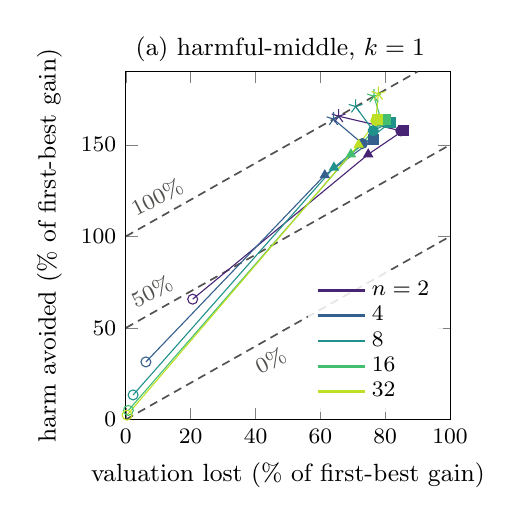
\begin{tikzpicture}
\begin{axis}[width=0.47\textwidth,height=6cm,xmin=0,xmax=100,ymin=0,ymax=190,
  xlabel={valuation lost (\% of first-best gain)},ylabel={harm avoided (\% of first-best gain)},
  title={(a) harmful-middle, $k=1$},every axis title/.style={at={(0,1)},anchor=south west,font=\small},
  legend style={at={(0.98,0.02)},anchor=south east,draw=none,fill=white,fill opacity=0.85,text opacity=1,font=\footnotesize,row sep=-1.5pt},legend cell align=left]
\addplot[ref line,domain=0:100,samples=2,forget plot]{x};
\addplot[ref line,domain=0:100,samples=2,forget plot]{x+50};
\addplot[ref line,domain=0:90,samples=2,forget plot]{x+100};
\node[font=\footnotesize,text=inksec,anchor=north west,rotate=27] at (axis cs:35,35) {$0\%$};
\node[font=\footnotesize,text=inksec,anchor=south west,rotate=27] at (axis cs:2,53) {$50\%$};
\node[font=\footnotesize,text=inksec,anchor=south west,rotate=27] at (axis cs:2,103) {$100\%$};
\addlegendimage{fiveA,line width=1pt}\addlegendentry{$n=2$}
\addlegendimage{fiveB,line width=1pt}\addlegendentry{$4$}
\addlegendimage{fiveC,line width=1pt}\addlegendentry{$8$}
\addlegendimage{fiveD,line width=1pt}\addlegendentry{$16$}
\addlegendimage{fiveE,line width=1pt}\addlegendentry{$32$}
\addplot[fiveA,thin,forget plot] coordinates {(20.61,65.71) (74.76,144.82) (85.52,157.75) (84.81,157.65) (65.63,165.63)};
\addplot[fiveA,only marks,mark=o,mark size=1.8pt,forget plot] coordinates {(20.61,65.71)};
\addplot[fiveA,only marks,mark=triangle*,mark size=1.8pt,forget plot] coordinates {(74.76,144.82)};
\addplot[fiveA,only marks,mark=square*,mark size=1.8pt,forget plot] coordinates {(85.52,157.75)};
\addplot[fiveA,only marks,mark=*,mark size=1.8pt,forget plot] coordinates {(84.81,157.65)};
\addplot[fiveA,only marks,mark=star,mark size=2.6pt,forget plot] coordinates {(65.63,165.63)};
\addplot[fiveB,thin,forget plot] coordinates {(6.18,31.43) (61.36,133.44) (76.44,152.81) (72.94,150.70) (64.04,164.04)};
\addplot[fiveB,only marks,mark=o,mark size=1.8pt,forget plot] coordinates {(6.18,31.43)};
\addplot[fiveB,only marks,mark=triangle*,mark size=1.8pt,forget plot] coordinates {(61.36,133.44)};
\addplot[fiveB,only marks,mark=square*,mark size=1.8pt,forget plot] coordinates {(76.44,152.81)};
\addplot[fiveB,only marks,mark=*,mark size=1.8pt,forget plot] coordinates {(72.94,150.70)};
\addplot[fiveB,only marks,mark=star,mark size=2.6pt,forget plot] coordinates {(64.04,164.04)};
\addplot[fiveC,thin,forget plot] coordinates {(2.23,13.40) (64.19,137.61) (81.56,162.26) (76.30,157.77) (70.87,170.87)};
\addplot[fiveC,only marks,mark=o,mark size=1.8pt,forget plot] coordinates {(2.23,13.40)};
\addplot[fiveC,only marks,mark=triangle*,mark size=1.8pt,forget plot] coordinates {(64.19,137.61)};
\addplot[fiveC,only marks,mark=square*,mark size=1.8pt,forget plot] coordinates {(81.56,162.26)};
\addplot[fiveC,only marks,mark=*,mark size=1.8pt,forget plot] coordinates {(76.30,157.77)};
\addplot[fiveC,only marks,mark=star,mark size=2.6pt,forget plot] coordinates {(70.87,170.87)};
\addplot[fiveD,thin,forget plot] coordinates {(0.77,4.96) (69.42,144.81) (79.97,164.04) (78.82,162.93) (76.53,176.53)};
\addplot[fiveD,only marks,mark=o,mark size=1.8pt,forget plot] coordinates {(0.77,4.96)};
\addplot[fiveD,only marks,mark=triangle*,mark size=1.8pt,forget plot] coordinates {(69.42,144.81)};
\addplot[fiveD,only marks,mark=square*,mark size=1.8pt,forget plot] coordinates {(79.97,164.04)};
\addplot[fiveD,only marks,mark=*,mark size=1.8pt,forget plot] coordinates {(78.82,162.93)};
\addplot[fiveD,only marks,mark=star,mark size=2.6pt,forget plot] coordinates {(76.53,176.53)};
\addplot[fiveE,thin,forget plot] coordinates {(0.36,2.38) (71.81,150.11) (77.58,163.67) (77.10,163.25) (77.88,177.88)};
\addplot[fiveE,only marks,mark=o,mark size=1.8pt,forget plot] coordinates {(0.36,2.38)};
\addplot[fiveE,only marks,mark=triangle*,mark size=1.8pt,forget plot] coordinates {(71.81,150.11)};
\addplot[fiveE,only marks,mark=square*,mark size=1.8pt,forget plot] coordinates {(77.58,163.67)};
\addplot[fiveE,only marks,mark=*,mark size=1.8pt,forget plot] coordinates {(77.10,163.25)};
\addplot[fiveE,only marks,mark=star,mark size=2.6pt,forget plot] coordinates {(77.88,177.88)};

\end{axis}
\end{tikzpicture}\hfill
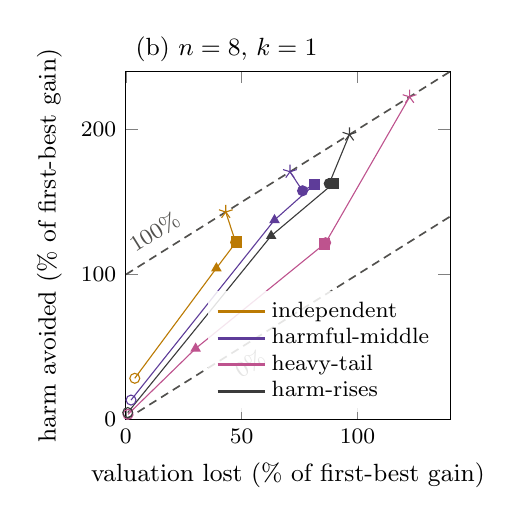
\begin{tikzpicture}
\begin{axis}[width=0.47\textwidth,height=6cm,xmin=0,xmax=140,ymin=0,ymax=240,
  xlabel={valuation lost (\% of first-best gain)},ylabel={harm avoided (\% of first-best gain)},
  title={(b) $n=8$, $k=1$},every axis title/.style={at={(0,1)},anchor=south west,font=\small},
  legend style={at={(0.98,0.02)},anchor=south east,draw=none,fill=white,fill opacity=0.85,text opacity=1,font=\footnotesize,row sep=-1.5pt},legend cell align=left]
\addplot[ref line,domain=0:140,samples=2,forget plot]{x};
\addplot[ref line,domain=0:140,samples=2,forget plot]{x+100};
\node[font=\footnotesize,text=inksec,anchor=north west,rotate=32] at (axis cs:40,40) {$0\%$};
\node[font=\footnotesize,text=inksec,anchor=south west,rotate=32] at (axis cs:3,105) {$100\%$};
\addlegendimage{seriesA,line width=1pt}\addlegendentry{independent}
\addlegendimage{seriesB,line width=1pt}\addlegendentry{harmful-middle}
\addlegendimage{seriesC,line width=1pt}\addlegendentry{heavy-tail}
\addlegendimage{seriesD,line width=1pt}\addlegendentry{harm-rises}
\addplot[seriesA,thin,forget plot] coordinates {(3.85,28.42) (39.09,104.34) (47.65,122.44) (47.41,122.20) (43.14,143.14)};
\addplot[seriesA,only marks,mark=o,mark size=1.8pt,forget plot] coordinates {(3.85,28.42)};
\addplot[seriesA,only marks,mark=triangle*,mark size=1.8pt,forget plot] coordinates {(39.09,104.34)};
\addplot[seriesA,only marks,mark=square*,mark size=1.8pt,forget plot] coordinates {(47.65,122.44)};
\addplot[seriesA,only marks,mark=*,mark size=1.8pt,forget plot] coordinates {(47.41,122.20)};
\addplot[seriesA,only marks,mark=star,mark size=2.6pt,forget plot] coordinates {(43.14,143.14)};
\addplot[seriesB,thin,forget plot] coordinates {(2.23,13.40) (64.19,137.61) (81.56,162.26) (76.30,157.77) (70.87,170.87)};
\addplot[seriesB,only marks,mark=o,mark size=1.8pt,forget plot] coordinates {(2.23,13.40)};
\addplot[seriesB,only marks,mark=triangle*,mark size=1.8pt,forget plot] coordinates {(64.19,137.61)};
\addplot[seriesB,only marks,mark=square*,mark size=1.8pt,forget plot] coordinates {(81.56,162.26)};
\addplot[seriesB,only marks,mark=*,mark size=1.8pt,forget plot] coordinates {(76.30,157.77)};
\addplot[seriesB,only marks,mark=star,mark size=2.6pt,forget plot] coordinates {(70.87,170.87)};
\addplot[seriesC,thin,forget plot] coordinates {(0.91,3.52) (30.12,48.96) (85.72,121.06) (86.27,121.93) (122.52,222.52)};
\addplot[seriesC,only marks,mark=o,mark size=1.8pt,forget plot] coordinates {(0.91,3.52)};
\addplot[seriesC,only marks,mark=triangle*,mark size=1.8pt,forget plot] coordinates {(30.12,48.96)};
\addplot[seriesC,only marks,mark=square*,mark size=1.8pt,forget plot] coordinates {(85.72,121.06)};
\addplot[seriesC,only marks,mark=*,mark size=1.8pt,forget plot] coordinates {(86.27,121.93)};
\addplot[seriesC,only marks,mark=star,mark size=2.6pt,forget plot] coordinates {(122.52,222.52)};
\addplot[seriesD,thin,forget plot] coordinates {(0.81,4.77) (62.74,126.68) (89.86,163.11) (87.82,162.75) (96.55,196.55)};
\addplot[seriesD,only marks,mark=o,mark size=1.8pt,forget plot] coordinates {(0.81,4.77)};
\addplot[seriesD,only marks,mark=triangle*,mark size=1.8pt,forget plot] coordinates {(62.74,126.68)};
\addplot[seriesD,only marks,mark=square*,mark size=1.8pt,forget plot] coordinates {(89.86,163.11)};
\addplot[seriesD,only marks,mark=*,mark size=1.8pt,forget plot] coordinates {(87.82,162.75)};
\addplot[seriesD,only marks,mark=star,mark size=2.6pt,forget plot] coordinates {(96.55,196.55)};

\end{axis}
\end{tikzpicture}\\[4pt]
\keylegend{\addlegendimage{ink,only marks,mark=o}\addlegendentry{$\tau^0$}
\addlegendimage{ink,only marks,mark=triangle*}\addlegendentry{best cutoff}
\addlegendimage{ink,only marks,mark=square*}\addlegendentry{best affine}
\addlegendimage{ink,only marks,mark=*}\addlegendentry{optimized $\tau$}
\addlegendimage{ink,only marks,mark=star,mark size=2.6pt}\addlegendentry{first best}}
\caption{Valuation lost and harm avoided relative to VCG, in percent of the first-best gain, for VCG-PA with each threshold function (marks, joined in the order $\tau^0$, best cutoff, best affine, optimized) and for the first best (star). Dashed diagonals: equal share of the first-best gain. (a) Harmful-middle, one good, by $n$; (b) every distribution at $n=8$, $k=1$.}
\label{fig:harm}
\end{figure}

\subsection{Simple Threshold Functions}\label{sec:forms}

\Cref{fig:share21,fig:share164} repeat Figure~3 of the paper, which shows $(n,k)=(8,1)$, for $(2,1)$ and $(16,4)$. The optimized $\tau$ is steeper than every welfare cutoff, whose lines have slope $-1$ in the type plane. The best affine $\tau$ follows the optimized $\tau$ over most types, and its share of the first-best gain is within $2.3$ pp of that of the optimized $\tau$ in every market and distribution (\cref{tab:harmful,tab:independent,tab:heavy,tab:rises}). In three markets with $n\geq16$ (harmful-middle $(32,2)$, independent $(16,1)$ and $(32,1)$), the best affine $\tau$ exceeds the result of threshold-response ascent by up to $0.4$ pp, so every start of the ascent ends at a local optimum there. The best cutoff loses up to $9$ pp in harmful-middle, $11$ pp in independent and harm-rises, and $25$ pp in heavy-tail.

\begin{figure}[htbp]
\centering
\sharefigure{2}{1}
\caption{$n=2$ bidders, $k=1$ good, as Figure~3 of the paper. (a) Welfare in percent of the first best $\FB$ by type distribution: VCG without audits (dashed line), VCG-PA with each threshold function, and IVCG-PA with $\tauea$ and with optimized $\tau$. Filled marks: optimized $\tau$; hollow marks: given or restricted $\tau$. Bar: the guarantee $\max\{\rho_{n,k},1-1/\eul\}\FB$ of IVCG-PA with $\tauea$. (b)--(e) The VCG-PA threshold functions over the type distribution (gray) of the column above.}
\label{fig:share21}
\end{figure}

\begin{figure}[htbp]
\centering
\sharefigure{16}{4}
\caption{$n=16$ bidders, $k=4$ goods; as \cref{fig:share21}.}
\label{fig:share164}
\end{figure}

\subsection{Optimized Threshold Functions and Penalties by Market}\label{sec:shapes}

\Cref{fig:taumarkets} shows the VCG-PA-optimized $\tau$ in two families of markets: one good with $n$ from $2$ to $32$ (a)--(d), and $n=16$ bidders with $k$ from $1$ to $14$ (e)--(h). Both families vary the number of bidders per good $n/k$, and in every distribution the optimized $\tau$ rises with $n/k$ in both. This is consistent with the rival welfare loss $L^\tau$: with more rivals per good, the good that a participant wins would more often go to a rival if the participant abstained, so a type needs a higher valuation to have positive marginal contribution. In independent, the optimized $\tau$ is nearly vertical: it excludes the most harmful externalities and admits the others at low thresholds.

\Cref{fig:penaltymarkets} shows the penalty functions $r(e)=\int_0^{\tau(e)}X^\tau$ of the same designs. A penalty is at most $\tau(e)$, and smaller where bids below $\tau(e)$ win less often. With more bidders per good, bids below a given $\tau(e)$ win less often, so the penalty is smaller relative to $\tau(e)$. In heavy-tail and independent, the penalties fall as $n/k$ grows; in harmful-middle and harm-rises, the penalty at a given externality rises with $n/k$ where $\tau$ rises, and the penalties of the excluded externalities change little.

\begin{figure}[htbp]
\centering
\begin{tikzpicture}
\begin{groupplot}[group style={group size=4 by 2,horizontal sep=\pg,vertical sep=1.65cm},row panel]
\formaxis{(a) independent}{Independent}{ylabel={valuation $v$}}\bgimage{Independent}{bg_independent}\byn{tau}{independent}\refline{Independent}
\formaxis{(b) harmful-middle}{HarmfulMiddle}{}\bgimage{HarmfulMiddle}{bg_harmful-middle}\byn{tau}{harmful-middle}\refline{HarmfulMiddle}
\formaxis{(c) heavy-tail}{HeavyTail}{}\bgimage{HeavyTail}{bg_heavy-tail}\byn{tau}{heavy-tail}\refline{HeavyTail}
\formaxis{(d) harm-rises}{HarmRises}{}\bgimage{HarmRises}{bg_harm-rises}\byn{tau}{harm-rises}\refline{HarmRises}
\formaxis{(e) independent}{Independent}{ylabel={valuation $v$}}\bgimage{Independent}{bg_independent}\byk{tau}{independent}\refline{Independent}
\formaxis{(f) harmful-middle}{HarmfulMiddle}{}\bgimage{HarmfulMiddle}{bg_harmful-middle}\byk{tau}{harmful-middle}\refline{HarmfulMiddle}
\formaxis{(g) heavy-tail}{HeavyTail}{}\bgimage{HeavyTail}{bg_heavy-tail}\byk{tau}{heavy-tail}\refline{HeavyTail}
\formaxis{(h) harm-rises}{HarmRises}{}\bgimage{HarmRises}{bg_harm-rises}\byk{tau}{harm-rises}\refline{HarmRises}
\end{groupplot}
\end{tikzpicture}\\[1pt]
\ratiolegend
\caption{VCG-PA-optimized threshold functions $\tau$ over the type distribution (gray), with the zero-welfare line $v=-e$ (thin dashed). (a)--(d) One good, $n\in\{2,4,8,16,32\}$ bidders; (e)--(h) $n=16$ bidders, $k\in\{1,2,4,8,12,14\}$ goods. Color and line style give the number of bidders per good $n/k$. A threshold at the top of a panel excludes the externality or is above the plotted valuations.}
\label{fig:taumarkets}
\end{figure}

\begin{figure}[htbp]
\centering
\begin{tikzpicture}
\begin{groupplot}[group style={group size=4 by 2,horizontal sep=\pg,vertical sep=1.65cm},row panel,ymin=0]
\formaxis{(a) independent}{Independent}{ylabel={penalty $r(e)$},ymin=0,ymax=1.05}\byn{r}{independent}
\formaxis{(b) harmful-middle}{HarmfulMiddle}{ymin=0,ymax=2.6}\byn{r}{harmful-middle}
\formaxis{(c) heavy-tail}{HeavyTail}{ymin=0,ymax=2.6}\byn{r}{heavy-tail}
\formaxis{(d) harm-rises}{HarmRises}{ymin=0,ymax=2.0}\byn{r}{harm-rises}
\formaxis{(e) independent}{Independent}{ylabel={penalty $r(e)$},ymin=0,ymax=1.05}\byk{r}{independent}
\formaxis{(f) harmful-middle}{HarmfulMiddle}{ymin=0,ymax=2.6}\byk{r}{harmful-middle}
\formaxis{(g) heavy-tail}{HeavyTail}{ymin=0,ymax=2.6}\byk{r}{heavy-tail}
\formaxis{(h) harm-rises}{HarmRises}{ymin=0,ymax=2.0}\byk{r}{harm-rises}
\end{groupplot}
\end{tikzpicture}\\[1pt]
\ratiolegend
\caption{Penalty functions $r(e)$ of the VCG-PA-optimized threshold functions of \cref{fig:taumarkets}, in valuation units. (a)--(d) One good, $n\in\{2,4,8,16,32\}$ bidders; (e)--(h) $n=16$ bidders, $k\in\{1,2,4,8,12,14\}$ goods. Excluded externalities get the penalty $\int_0^{\bar v}X^\tau$.}
\label{fig:penaltymarkets}
\end{figure}

\subsection{Marginal Contributions and Pigouvian Penalties}\label{sec:marginal}

By Section~6.3, at an optimal $\tau$ the threshold type of each interior threshold has zero marginal contribution $M^\tau(e,v)=(v+e)X^\tau(v)-L^\tau(v)$, and its penalty equals the Pigouvian charge $-eX^\tau+L^\tau-P^\tau$. \Cref{fig:marginal} shows both at $(n,k)=(8,1)$. In every distribution, the optimized $\tau$ is close to the zero contour of $M^\tau$ where $\tau$ is interior, so the participants are almost exactly the types with positive marginal contribution; where the two curves differ, as in harmful-middle at valuations below about $1.1$, $M^\tau$ is close to $0$. At the interior thresholds, the penalty and the Pigouvian charge differ by at most $2.3\cdot10^{-6}$ in harmful-middle, $1.5\cdot10^{-8}$ in independent, $1.9\cdot10^{-5}$ in harm-rises and $4.9\cdot10^{-3}$ in heavy-tail, with penalties up to $2.5$.

\begin{figure}[htbp]
\centering
\begin{tikzpicture}
\begin{groupplot}[group style={group size=4 by 2,horizontal sep=0.7cm,vertical sep=1.5cm},
  scale only axis,width=\pw,height=2.6cm,xlabel={externality $e$},axis on top,
  every axis title/.style={at={(0,1)},anchor=south west,font=\small},xlabel style={yshift=2pt}]
\nextgroupplot[title={(a) independent},ylabel={valuation $v$},xmin=\eminMapIndependent,xmax=\emaxMapIndependent,ymin=\vminMapIndependent,ymax=\vmaxMapIndependent]
\mapimage{Independent}{mc_independent}
\addplot[main curve,forget plot,unbounded coords=jump] table[x=e,y=tau]{data/tau_mc_independent.dat};
\nextgroupplot[title={(b) harmful-middle},xmin=\eminMapHarmfulMiddle,xmax=\emaxMapHarmfulMiddle,ymin=\vminMapHarmfulMiddle,ymax=\vmaxMapHarmfulMiddle]
\mapimage{HarmfulMiddle}{mc_harmful-middle}
\addplot[main curve,forget plot,unbounded coords=jump] table[x=e,y=tau]{data/tau_mc_harmful-middle.dat};
\nextgroupplot[title={(c) heavy-tail},xmin=\eminMapHeavyTail,xmax=\emaxMapHeavyTail,ymin=\vminMapHeavyTail,ymax=\vmaxMapHeavyTail]
\mapimage{HeavyTail}{mc_heavy-tail}
\addplot[main curve,forget plot,unbounded coords=jump] table[x=e,y=tau]{data/tau_mc_heavy-tail.dat};
\nextgroupplot[title={(d) harm-rises},xmin=\eminMapHarmRises,xmax=\emaxMapHarmRises,ymin=\vminMapHarmRises,ymax=\vmaxMapHarmRises]
\mapimage{HarmRises}{mc_harm-rises}
\addplot[main curve,forget plot,unbounded coords=jump] table[x=e,y=tau]{data/tau_mc_harm-rises.dat};
\nextgroupplot[title={(e) independent},ylabel={penalty, charge},xmin=\eminMapIndependent,xmax=\emaxMapIndependent,ymin=0]
\addplot[main curve] table[x=e,y=penalty]{data/pigou_independent.dat};
\addplot[seriesA,only marks,mark=o,mark size=1.4pt,line width=0.7pt,each nth point=3] table[x=e,y=charge]{data/pigou_independent.dat};
\nextgroupplot[title={(f) harmful-middle},xmin=\eminMapHarmfulMiddle,xmax=\emaxMapHarmfulMiddle,ymin=0]
\addplot[main curve] table[x=e,y=penalty]{data/pigou_harmful-middle.dat};
\addplot[seriesA,only marks,mark=o,mark size=1.4pt,line width=0.7pt,each nth point=3] table[x=e,y=charge]{data/pigou_harmful-middle.dat};
\nextgroupplot[title={(g) heavy-tail},xmin=\eminMapHeavyTail,xmax=\emaxMapHeavyTail,ymin=0]
\addplot[main curve] table[x=e,y=penalty]{data/pigou_heavy-tail.dat};
\addplot[seriesA,only marks,mark=o,mark size=1.4pt,line width=0.7pt,each nth point=3] table[x=e,y=charge]{data/pigou_heavy-tail.dat};
\nextgroupplot[title={(h) harm-rises},xmin=\eminMapHarmRises,xmax=\emaxMapHarmRises,ymin=0]
\addplot[main curve] table[x=e,y=penalty]{data/pigou_harm-rises.dat};
\addplot[seriesA,only marks,mark=o,mark size=1.4pt,line width=0.7pt,each nth point=3] table[x=e,y=charge]{data/pigou_harm-rises.dat};
\end{groupplot}
\end{tikzpicture}\\[1pt]
\keylegend{\addlegendimage{area legend,draw=none,fill=mcpos}\addlegendentry{$M^\tau>0$}
\addlegendimage{area legend,draw=none,fill=mcneg}\addlegendentry{$M^\tau<0$}
\addlegendimage{ink,line width=0.9pt,densely dashed}\addlegendentry{$M^\tau=0$}
\addlegendimage{inksec,line width=0.6pt}\addlegendentry{edge of the type distribution}}\\
\keylegend{\addlegendimage{main curve}\addlegendentry{$\tau$ in (a)--(d), penalty $r(e)$ in (e)--(h)}
\addlegendimage{seriesA,only marks,mark=o,mark size=1.4pt,line width=0.7pt}\addlegendentry{Pigouvian charge}}
\caption{VCG-PA with optimized $\tau$, $n=8$, $k=1$. (a)--(d) Marginal contribution $M^\tau(e,v)$ (symmetric logarithmic color scale; darker is larger in absolute value) with its zero contour and the optimized $\tau$. (e)--(h) Penalty $r(e)$ and the Pigouvian charge $-eX^\tau+L^\tau-P^\tau$ of the threshold type, at every third externality node with an interior threshold. Exact.}
\label{fig:marginal}
\end{figure}

\subsection{Ironing}\label{sec:ironing}

Ironing binds at the optimized $\tau$ only in harmful-middle, and IVCG-PA adds the most there at $(n,k)=(2,1)$. \Cref{fig:ironing} shows this design. The expected welfare contribution $\hat w^\tau$ of a participant rises with the bid up to about $0.8$, falls to a minimum at about $1.3$, where the conditional mean externality falls faster than the valuation rises, and rises again (b). IVCG-PA pools all bids above $\ironpoolstart$: they get one score, the mean of $\hat w^\tau$ over the pool, and two participants with pooled bids are ranked by the tie-breaking lottery. The interim allocation of IVCG-PA is therefore constant on the pool (c). Compared with the VCG-PA-optimized $\tau$, the IVCG-PA-optimized $\tau$ is lower by about $0.1$ at externalities below $-0.4$, so that IVCG-PA admits more of the harmful types with high valuations, and higher at externalities around $-0.3$ (a).

\begin{figure}[htbp]
\centering
\begin{tikzpicture}
\begin{groupplot}[group style={group size=3 by 1,horizontal sep=1.3cm},
  scale only axis,width=4.1cm,height=3.3cm,axis on top,
  every axis title/.style={at={(0,1)},anchor=south west,font=\small}]
\nextgroupplot[title={(a) optimized $\tau$},xlabel={externality $e$},ylabel={valuation $v$},
  xmin=\eminHarmfulMiddle,xmax=\emaxHarmfulMiddle,ymin=\vminHarmfulMiddle,ymax=\vmaxHarmfulMiddle]
\addplot[draw=none,fill=regionqty,forget plot] table[x=e,y expr={max(min(\thisrow{ivcgpa},\vmaxHarmfulMiddle),\ironpoolstart)}]{data/iron_tau.dat} -- (axis cs:\emaxImgHarmfulMiddle,\vmaxHarmfulMiddle) -- (axis cs:\eminImgHarmfulMiddle,\vmaxHarmfulMiddle) -- cycle;
\bgimage{HarmfulMiddle}{bg_harmful-middle}
\refline{HarmfulMiddle}
\addplot[vcgpa,line width=1.4pt,forget plot] table[x=e,y=vcgpa]{data/iron_tau.dat};
\addplot[ivcgpa,line width=1.2pt,dashed,forget plot] table[x=e,y=ivcgpa]{data/iron_tau.dat};
\nextgroupplot[title={(b) scores},xlabel={bid $b$},ylabel={welfare contribution},xmin=0,xmax=\vmaxHarmfulMiddle]
\fill[regionqty] ({axis cs:0.0079678,0}|-{rel axis cs:0,0}) rectangle ({axis cs:0.032051,0}|-{rel axis cs:0,1});
\fill[regionqty] ({axis cs:0.60844,0}|-{rel axis cs:0,0}) rectangle ({axis cs:2.1034,0}|-{rel axis cs:0,1});

\addplot[main curve,forget plot] table[x=b,y=what]{data/iron_scores.dat};
\addplot[ivcgpa,line width=1.2pt,dashed,forget plot] table[x=b,y=wbar]{data/iron_scores.dat};
\nextgroupplot[title={(c) interim allocation},xlabel={bid $b$},ylabel={$X^\tau(b)$},xmin=0,xmax=\vmaxHarmfulMiddle,ymin=0,ymax=1.02]
\fill[regionqty] ({axis cs:0.0079678,0}|-{rel axis cs:0,0}) rectangle ({axis cs:0.032051,0}|-{rel axis cs:0,1});
\fill[regionqty] ({axis cs:0.60844,0}|-{rel axis cs:0,0}) rectangle ({axis cs:2.1034,0}|-{rel axis cs:0,1});

\addplot[vcgpa,line width=1.4pt,forget plot] table[x=b,y=vcgpa]{data/iron_alloc.dat};
\addplot[ivcgpa,line width=1.2pt,dashed,forget plot] table[x=b,y=ivcgpa]{data/iron_alloc.dat};
\end{groupplot}
\end{tikzpicture}\\[1pt]
\keylegend{\addlegendimage{vcgpa,line width=1.4pt}\addlegendentry{VCG-PA}
\addlegendimage{ivcgpa,line width=1.2pt,dashed}\addlegendentry{IVCG-PA}
\addlegendimage{main curve}\addlegendentry{expected welfare contribution $\hat w^\tau$}
\addlegendimage{area legend,draw=none,fill=regionqty}\addlegendentry{pooled bids}}
\caption{Harmful-middle, $n=2$, $k=1$. (a) The VCG-PA-optimized and the IVCG-PA-optimized $\tau$ over the type distribution (gray), with the zero-welfare line (thin dashed) and the valuations pooled by IVCG-PA. (b) For the IVCG-PA-optimized $\tau$: the expected welfare contribution $\hat w^\tau(b)$ of a participant with bid $b$, and the IVCG-PA score $\bar\omega^\tau(b)$ (dashed), constant on the pooled bids. (c) The interim allocations $X^\tau$ of VCG-PA and IVCG-PA with the IVCG-PA-optimized $\tau$. Exact.}
\label{fig:ironing}
\end{figure}

\subsection{Revenue, Penalties and Participation}\label{sec:revenue}

\Cref{tab:money} reports, for VCG-PA with optimized $\tau$, the auction revenue and the penalties paid as a share of VCG revenue, the bidders' net utility as a share of their net utility under VCG, and the expected share of bidders that participate. In every listed market, the auction revenue of VCG-PA is below that of VCG, since fewer bidders participate. In harmful-middle, where the excluded harmful types have high valuations, the revenue falls to $28$--$39\%$ of VCG revenue in the markets with $n/k\geq2$ and to $10$--$24\%$ in those with $k/n\geq3/4$; penalties recover up to $26\%$ of VCG revenue at $n/k\geq2$ and $47$--$77\%$ at $k/n\geq3/4$. Bidders' net utility is $73$--$116\%$ of its VCG level, and $11$--$81\%$ of bidders participate. The optimized $\tau$ maximizes welfare and ignores revenue.

\begin{table}[htbp]
\centering\footnotesize
\begin{tabular}{@{}lrrrrrrrr@{}}
\toprule
 & & & VCG & \multicolumn{5}{c}{VCG-PA with optimized $\tau$}\\
\cmidrule(l){5-9}
distribution & $n$ & $k$ & revenue & revenue & penalties & rev.\,+\,pen. & net utility & participants\\
\midrule
\multirow{8}{*}{independent} & 2 & 1 & 0.33 & 36.7 & 27.7 & 64.4 & 86.1 & 54.0 \\
 & 8 & 1 & 0.78 & 50.6 & 2.6 & 53.2 & 243.3 & 32.0 \\
 & 32 & 1 & 0.94 & 61.3 & 0.4 & 61.7 & 679.2 & 13.6 \\
 & 8 & 2 & 1.33 & 43.0 & 9.2 & 52.2 & 175.5 & 39.2 \\
 & 16 & 4 & 2.82 & 40.7 & 11.1 & 51.7 & 201.8 & 35.9 \\
 & 32 & 8 & 5.82 & 37.2 & 14.5 & 51.7 & 218.8 & 33.0 \\
 & 4 & 3 & 0.60 & 18.5 & 61.1 & 79.6 & 74.3 & 59.7 \\
 & 16 & 14 & 1.65 & 0.7 & 109.7 & 110.4 & 67.1 & 63.2 \\
\midrule
\multirow{8}{*}{harmful-middle} & 2 & 1 & 0.77 & 31.2 & 26.1 & 57.3 & 81.9 & 61.5 \\
 & 8 & 1 & 1.39 & 34.1 & 3.9 & 37.9 & 114.3 & 29.5 \\
 & 32 & 1 & 1.74 & 37.2 & 0.6 & 37.8 & 104.5 & 11.4 \\
 & 8 & 2 & 2.44 & 33.4 & 9.1 & 42.4 & 112.8 & 40.3 \\
 & 16 & 4 & 5.05 & 33.1 & 10.0 & 43.1 & 114.3 & 36.7 \\
 & 32 & 8 & 10.28 & 32.0 & 11.9 & 43.9 & 114.3 & 33.7 \\
 & 4 & 3 & 1.72 & 23.9 & 48.7 & 72.6 & 76.4 & 72.2 \\
 & 16 & 14 & 6.42 & 10.4 & 74.0 & 84.4 & 79.2 & 80.7 \\
\midrule
\multirow{8}{*}{heavy-tail} & 2 & 1 & 0.78 & 71.8 & 53.9 & 125.7 & 82.0 & 74.1 \\
 & 8 & 1 & 2.58 & 92.8 & 12.2 & 105.0 & 90.6 & 53.4 \\
 & 32 & 1 & 5.18 & 98.3 & 3.3 & 101.6 & 95.0 & 31.8 \\
 & 8 & 2 & 3.50 & 85.7 & 23.1 & 108.7 & 87.6 & 57.9 \\
 & 16 & 4 & 7.37 & 84.0 & 24.8 & 108.8 & 87.1 & 51.3 \\
 & 32 & 8 & 15.13 & 81.3 & 27.8 & 109.1 & 86.5 & 45.5 \\
 & 4 & 3 & 1.35 & 46.8 & 105.3 & 152.1 & 78.6 & 76.8 \\
 & 16 & 14 & 4.20 & 13.5 & 166.6 & 180.1 & 77.9 & 79.8 \\
\midrule
\multirow{8}{*}{harm-rises} & 2 & 1 & 0.79 & 54.2 & 27.2 & 81.4 & 92.5 & 75.0 \\
 & 8 & 1 & 1.34 & 57.3 & 10.2 & 67.5 & 119.8 & 39.2 \\
 & 32 & 1 & 1.66 & 53.8 & 9.4 & 63.2 & 115.2 & 15.7 \\
 & 8 & 2 & 2.38 & 55.0 & 14.7 & 69.7 & 116.7 & 48.5 \\
 & 16 & 4 & 4.92 & 52.2 & 17.4 & 69.6 & 115.5 & 42.3 \\
 & 32 & 8 & 10.01 & 48.5 & 21.2 & 69.7 & 112.4 & 37.3 \\
 & 4 & 3 & 1.82 & 45.0 & 46.5 & 91.5 & 86.1 & 82.2 \\
 & 16 & 14 & 7.03 & 28.6 & 69.4 & 98.0 & 86.5 & 86.9 \\
\bottomrule
\end{tabular}

\caption{VCG-PA with optimized $\tau$ in eight markets of each distribution: VCG revenue (level); auction revenue, penalties paid, and their sum, in percent of VCG revenue; bidders' net utility in percent of its VCG level; participants in percent of $n$. Exact.}
\label{tab:money}
\end{table}

\subsection{Convergence and Local Optima}\label{sec:local}

In $159$ of the $160$ designs computed by threshold-response ascent, all nine starts reach the same welfare within $1.1\cdot10^{-6}$ of the first-best gain $\FB-\W_0$. In harmful-middle at $(32,8)$, VCG-PA, the starts reach two local optima, $1.8\cdot10^{-4}$ of the first-best gain apart, and the higher is kept. The relaxation start converges to the lower one there. Every search stage converged before its iteration cap and the time limit.

\section{Limitations of the Methods}\label{sec:limitations}

\begin{itemize}
    \item \emph{Discretization.} The search is exact for the piecewise-uniform distribution, which approximates each continuous density; $\tau$ is optimal for the grid, and is evaluated on the continuous version. The grid-refinement check bounds the resulting error, except in the heavy-tail markets listed in \cref{sec:experiment}.
    \item \emph{Local optima.} Threshold-response ascent and the grid searches find local optima of a nonconcave objective. Nine starts reduce this risk, but do not remove it: in three markets, the best affine $\tau$ exceeds the result of the ascent.
    \item \emph{Equal threshold functions.} All designs give every bidder the same $\tau$. Unequal threshold functions can have higher welfare (Example~6.1), so the reported shares of optimized designs are lower bounds on what the best threshold profile attains.
    \item \emph{Synthetic distributions.} The four distributions are chosen to vary the dependence between valuation and externality; they are not estimated from data.
\end{itemize}

\bibliographystyle{plainnat}
\bibliography{references}

\end{document}
